% REMEMBER: You must not plagiarise anything in your report. Be extremely careful.
\documentclass{l4proj}

    
%==============================================================================
% Put any additional packages here
% You can add any packages you want, as long as it does not alter
% the overall format (e.g. don't change the margins or the reference style).
%
\usepackage{pdfpages} % if you want to include a PDF for an ethics checklist, for example
\usepackage{wrapfig}
\usepackage{booktabs}
\usepackage{capt-of}
\usepackage[section]{placeins}
\usepackage{float}
%
%

\begin{document}

%==============================================================================
%% METADATA
\title{Health Misinformation, Covid-19, and Search} % change this to your title
\author{Shahzeb Zafar}
\date{April 7, 2022}

\maketitle

%==============================================================================
%% ABSTRACT
\begin{abstract}
    We are interested in knowing the characteristics of misinformation and whether it will decrease overtime with Covid-19 as the topic. By performing binary classification, sentiment and emotion analysis on Covid-19 tweets we discovered that misinformation does decrease over time and is characterised by negative and neutral sentiments, fear, anger, and disgust.
\end{abstract}

%==============================================================================
%% ACKNOWLEDGEMENTS
\chapter*{Acknowledgements}
% Enter any acknowledgements here. This is optional; you may leave this blank if you wish,
% or remove the entire chapter
%
% We give thanks to the Gods of LaTeX, who in their eternal graciousness, 
% have granted that this document may compile without errors or overfull hboxes.
%
I would like to thank Dr. Jesus Rodriguez Perez for being a great supervisor and helping me throughout the course of the project despite his own commitments and struggles. I also appreciate Head of Level 4 Projects Dr. Graham McDonalad and my Student Support Officer Una Marie Darragh for granting me an extension in light of my carpal tunnel syndrome.

%==============================================================================

% EDUCATION REUSE CONSENT FORM
% If you consent to your project being shown to future students for educational purposes
% then insert your name and the date below to  sign the education use form that appears in the front of the document. 
% You must explicitly give consent if you wish to do so.
% If you sign, your project may be included in the Hall of Fame if it scores particularly highly.
%
% Please note that you are under no obligation to sign 
% this declaration, but doing so would help future students.
%
%\def\consentname {My Name} % your full name
%\def\consentdate {20 March 2018} % the date you agree
%
\educationalconsent


%==============================================================================
\tableofcontents

%==============================================================================
%% Notes on formatting
%==============================================================================
% The first page, abstract and table of contents are numbered using Roman numerals and are not
% included in the page count. 
%
% From now on pages are numbered
% using Arabic numerals. Therefore, immediately after the first call to \chapter we need the call
% \pagenumbering{arabic} and this should be called once only in the document. 
%
%
% The first Chapter should then be on page 1. 

% PAGE LIMITS
% You are allowed 40 pages for a 40 credit project and 30 pages for a 
% 20 credit report. 
% This includes everything numbered in Arabic numerals (excluding front matter) up
% to but *excluding the appendices and bibliography*.
%
% FORMATTING
% You must not alter text size (it is currently 10pt) or alter margins or spacing.
% Do not alter the bibliography style. 
%
%==================================================================================================================================
%
% IMPORTANT
% The chapter headings and structure here are **suggestions**. You don't have to follow this model if
% it doesn't fit your project. Every project should have an introduction and conclusion,
% however.  If in doubt, your supervisor can give you specific guidance; their view takes precedence over
% the structure suggested here.
%
%==================================================================================================================================
\chapter{Introduction}

% reset page numbering. Don't remove this!
\pagenumbering{arabic} 

% You can use \todo{} to mark text that needs to be fixed. Anything inside will appear as highlighted 
% text in the final copy, and you will also get warnings when you compile (so you don't
% forget to take them out!)



We live in an age where digital information is a precious commodity. Governments use it in rapid decision making; corporations use it to generate profit, and ordinary people make use of such information to facilitate their day-to-day lives.

An area where digital information is of vital importance is the public health sector. The ability to diagnose common illnesses and find suitable treatments without having to visit the doctor is phenomenal. It not only saves money on medical bills, but also frees up the health services to handle more serious ailments.

However, health information, like any other information, is susceptible to falsification, particularly on the world wide web where millions upon millions of people partake in information exchange and discussions daily. This misinformation can spread rapidly and is detrimental to the overall welfare of people around the globe.

For instance, say a person suffering from allergies of some kind goes online to look for appropriate medication instead of consulting their GP. There are hundreds of non-prescription medicines available on the market and the person decides to follow the advice of an online article and purchase a few of them. However, instead of helping them, the medicine instead makes their condition worse. This is the result of following unreliable information from an unverified source.

Anyone can be a victim of misinformation so it is vital we understand what exactly constitutes it and come up with effective strategies to combat it. This is especially true for Covid-19 - a global pandemic affecting the lives of billions. There is plenty of confusion surrounding the virus which is made worse by the plethora of fake news about it.

Hence the goal of this project is to understand the scope of health misinformation floating online with Covid-19 as the topic of interest. We will analyse various trends and characteristics of this misinformation and see how it changes with the passage of time in hopes of understanding how and where such false information arises so that we may devise ways of limiting its exposure to ordinary people. 


%==================================================================================================================================
\chapter{Project Aims}
In this chapter we will define our research question, hypothesis and the steps to take to answer and prove them.

\section{Original Proposal}
First we'll take proper look at the original proposal for the project before breaking it down. The proposal is:

\vspace{0.4cm}
\begin{center}
    As the pandemic progresses, another pandemic has emerged as fake news and misinformation plagues the media. The most common way people gather information to understand a topic, is by searching in an ad-hoc manner (query for documents on a search engine). But a question arises: Which sources are the most reliable for a particular topic in a quickly developing event?Using the COVID pandemic as a use case can we evaluate and/or develop ways to find and make sense of this rapidly changing information?
\end{center}
\vspace{0.4cm}

Looking at the proposal, it is clear we're being asked to analyse the way the nature of misinformation changes over time in ad-hoc or exhaustive searches in regards to Covid-19. Our task involves gathering data people would stumble upon via a search engine e.g social media posts, and use it to characterise misinformation.

\section{Research Question and Hypothesis}
Our research question for the project is as follows:

\vspace{0.4cm}
\begin{center}
    "To what extent does the passage of time affect the quantity of misinformation floating online? And what are the identifying characteristics of such information?"
\end{center}
\vspace{0.4cm}

We went to know whether the amount of misinformation people can come across decrease as time goes on and more accurate information becomes available. Which leads us to our hypothesis:

\vspace{0.4cm}
\begin{center}
    "With the passage of time, information regarding any topic will increase in quantity, and there will be a noticeable improvement in its accuracy and authenticity with this increased volume."
\end{center}
\vspace{0.4cm}

And in order to combat misinformation, we definitely need to know the characteristics which make it up. Things such as when false information decreases or increases and by what amount; the underlying sentiment behind it; and the emotions associated with it are all things we are interested in.

\section{Steps to be Taken}
The steps to take to fulfill the goals of this project are:

\vspace{0.4cm}
\begin{enumerate}
    \item
    Gather Covid-19 data from some social media or search platform.
    \item
    Classify the data as either true or false.
    \item
    Separate the data into groups based on topics.
    \item
    Carry out sentiment analysis.
    \item
    Classify the underlying emotion in each instance of data.
    \item
    Visualise the results using appropriate means and analysing them.
\end{enumerate}
\vspace{0.4cm}

For the first step, we have decided to go with Twitter data due to the ease of using the Twitter API and the large datasets readily available online. Our aim for the project is to have around a million tweets for evaluation. Steps 2, 4 and 5 a classification tasks which can carried out by a NLP model such as BERT while step 3 would involve clustering of some sort.

%==================================================================================================================================
\chapter{Background}

There has been a lot of work done in the field of fake news detection, especially when it comes to Twitter data. One of the most important works in recent history has to be the efforts of \cite{banda_juan_m_2021_5652342} who have gathered over a billion tweets related to Covid-19 for research purposes. The team has worked with multiple collaborators worldwide to gather this data for public welfare and have continued to update it at the time of writing this paper.

For detecting fake news on Twitter, \cite{ATODIRESEI2018451} devised a very simple but effective approach in which they assigned a credibility score to tweets by comparing them to trustworthy news sources and also taking the credibility of the user itself into account, so the main goal is not the credibility of the tweets itself but rather the person who wrote it. Their application goes over the tweets of a user and compares them to legitimate sources to build up a user credibility score, and whenever said user posts a new tweet this score will greatly impact its credibility. However, there are some downsides to this approach. What guarantee is there that the trustworthy sources aren't full of fake news themselves?

Another novel approach comes from \cite{inbook} who used propagation graphs to train classifier and deep learning models to understand how real and fake news spread on Twitter. The idea is to examine how frequently a tweet gets retweeted, the retweets get retweeted, and so forth to observe how fast and far news spreads. According to their findings, fakes news spreads far faster and deeper than real news in most cases. However, this doesn't characterise fake news itself, at least not completely. \cite{lan9199} in their paper uses sentiments to identify fake news in Covid-19 tweets using NLP, which is very similar to what we're trying to achieve.

The recent works of \cite{jaimemv} and \cite{muller2020covid} also show very promising results for Covid-19 misinformation detection on Twitter. The former utilises simple BERT models and trains them to identify tweets as real or fake before making predictions on the dataset created by \cite{banda_juan_m_2021_5652342}, while the latter has trained a more complex BERT-large model with over a billion Covid-19 tweets and keeps finetuning the model with new tweets in order to make accurate predictions about fake news.

Using sentiments to characterise misinformation is commonplace these days. One of the earlier works is by \cite{Sarlan2014TwitterSA} who utilised various techniques to develop a machine learning models to classify sentiments of tweets. They put an extra emphasis on the quality of the training data rather than quantity since a larger volume of bad data made the models perform worse.

Building upon the above are the works by \cite{Roy2017ANS} and \cite{Gound2018TwitterDS}. The former developed a new method involving support vector machines (SVM) to predict positive and negative sentiments with a high degree of accuracy. The latter combines lexicon and machine learning-based approaches to sentiment classification and combines the best aspects of both to develop a sentiment analysis system that boasts superior accuracy over standard machine learning approaches. Both of these works served as prototypes for the more advanced techniques we use today.

In recent times, sentiment analysis is commonly accompanied by emotion analysis. In their work, \cite{SAILUNAZ2019101003} used the tried and tested Naive Bayes classifier to analyse Twitter data and find the underlying sentiments and emotions of tweets. Their approach was good for the time but since then we've had great advancements in the field of AI and the work of \cite{inproceedings} is a testament to this. By using BERT, they were able to predict the sentiments and emotions with over 90\% accuracy. \cite{perez2021pysentimiento} took this a step further and created an easy-to-use toolkit with a series of analysers and pre-trained models for Twitter sentiment and emotion analysis.

All of the above is useless if cannot effectively split tweets into groups. \cite{Sechelea2016TwitterDC} developed a system of harvesting twitter data, splitting it into clusters, and then visualising it using various 2D and 3D visualisation techniques. They used the unsupervised clustering techniques K-means and DBSCAN and combined the clusters using consensus clustering to take advantage of the benefits of both approaches. The work of \cite{Baralis2013AnalysisOT} goes for a similar approach but instead of combining different clustering techniques, they perform multi-level clustering by using the same clustering approach multiple times to get sub-clusters for a more thorough analysis of Twitter data. \cite{Alnajran2017ClusterAO} evaluated and compared various clustering approaches in their work to provide a compact review of them.

A breakthrough in clustering comes from the work of \cite{McConville2020} who created a simple deep clustering model by combining deep and shallow clustering techniques with local manifold learning. The N2D model has the advantage of speed over clustering approaches via deep learning, but at the same time, it vastly outperforms unsupervised and standard supervised approaches and was extremely competitive with state-of-the-art deep clustering algorithms at the time of publishing.



%==================================================================================================================================

\chapter{Methodology}
In this chapter we will go over the steps we took over the course of the project.

\section{Data Collection}
Since we decided to use Twitter data, one of the first things we did was take a look at the Twitter API. The API is feature-rich and provides many tools for accessing various aspects of Twitter data such as tweet text, location, username, date, etc. For our use case, we only needed the text of Covid-19 related tweets and the date they were published. However, the free version of the API has strict rate limits, and the developer account we had came with a limit of 250k tweets per month so it would take too long to gather data using it without having to pay over \pounds100 pm for a couple of months to get enough data for reasonable evaluation, something which was not feasible.

So instead we turned to Kaggle and explored the various Covid-19 datasets it had. Unlike with Twitter, we could access plenty of data however not all of it was relevant for what we needed and all the data we needed combined still fell short of our goal of 1 million tweets. Various repositories on GitHub also had what we needed but we ran into the same issues as Kaggle.

In the end, we found a large Covid-19 twitter dataset for scientific research by  \cite{banda_juan_m_2021_5652342} on Zenodo which contains tweet ids for millions upon millions of tweets. We used version 87 of the dataset which included ids and dates for tweets up until the start of November 2021. For this project, we decided to analyse tweets for January, April, July, and October for years 2020 and 2021. This period provided enough coverage for the pandemic and will, crucially, allow us to observe the change in tends and characteristics of misinformation for the twitter data.

Therefore we extracted 150,000 tweets for each of the periods mentioned above and used the Twitter hydrator by  \cite{hydrator} to convert the tweet ids into csv files containing all the data regarding the tweets. After keeping only the text and discarding the rest, we had a csv file for each period and around 1 million tweets overall.

\section{True/False Classification}
Classifying the data as either real or fake falls into the binary classification category. There are many ways of doing such tasks with Machine Learning and Deep Learning. We could either train a classifier from scratch, build a neural network, or use a pre-trained model. Websites such as GeeksforGeeks and Medium provide many tutorials on how to do binary classification but we were looking for something a bit more specialised.

One of the first sources we came across near the start of the project is the GitHub repository of  \cite{fnpcovid} who had his own annotated tweet data for training and was using the same Zenodo dataset as us for fake news prediction. It was a very fortunate find since the repository could be used to do the binary classification task with ease. However, the author was training a standard BERT model from scratch using tweets from early on in the pandemic. This presented an issue for us since we planned to make predictions for tweets from a much later period so his approach would not have been quite as good.

Thankfully, by following his citations, we came across a pre-trained BERT model by  \cite{muller2020covid} called Covid-Twitter-Bert-v2, which was trained using over 97M unique tweets and 1.2B training examples specifically for Covid-19. At the time when we used the model, the latest version had been trained using tweets up until August 2021 so it was perfect for our intended use case as the performance would be good for all of the time periods. Their GitHub repository had notebooks for finetuning the model so after converting them to run on our local machine instead of Google Colab, and using the training dataset provided by Muñoz, we were able to successfully classify 1M tweets as either true or false.

Table \ref{tab:train} summarises the results of the training process after 3 epochs for four models. By using the dataset of \cite{fnpcovid}, we can see that the pre-trained model scores highest across the board. The other models also had good performances however, they were trained from scratch and are not as complex as the pre-trained model (BERT-base vs BERT-large) so for the sake of better performance down the line, Covid-Twitter-Bert-v2 is our model of choice.

\begin{table}[h]
\centering
\begin{tabular}[width=1.0\linewidth]{lcccc}
                      & \multicolumn{1}{l}{Precision} & \multicolumn{1}{l}{Recall} & \multicolumn{1}{l}{F1-Score} & \multicolumn{1}{l}{Accuracy} \\
Covid-Twitter-Bert-v2 & 0.983                         & 0.985                      & 0.984                        & 0.984                        \\
Bert-Base-Cased       & 0.950                         & 0.952                      & 0.951                        & 0.953                        \\
Roberta-Base          & 0.952                         & 0.955                      & 0.953                        & 0.955                        \\
Albert-Base-v2        & 0.927                         & 0.931                      & 0.929                        & 0.932                       
\end{tabular}
\caption{Performance of different classification models. The values are macro averages.}
\label{tab:train}
\end{table}

\section{Data Clustering}
Clustering the tweets into topics proved to be the biggest challenge - on which we spent most of our time on. Popular clustering approaches like K-means and Spectral clustering would have worked but they're unsupervised approaches in which one would have to thoroughly analyse each cluster to determine the topic with no guarantee that a tweet will get assigned the same topic if the clustering were to be run again.

The plan was to split the tweets into 15 topics, and have the ability to assign new tweets topics without having to re-create the clusters. The work done by the likes of  \cite{Alnajran2017ClusterAO},  \cite{pksohn}, and  \cite{Sechelea2016TwitterDC} is all good for the unsupervised approach but it doesn't help with what we wanted to do. And for supervised methods, we created a basic annotated dataset by extracting a subset of tweets based on the words they contained and used it to train popular models like DeepCluster and DCN but the performance was just not good enough.

We then tried to use the pre-trained BERT model that we'd used for the binary classification as a substitute for clustering since at the end of the day, clustering is similar to multi-label classification. However, that model had been optimised for around a maximum of 5-6 labels and had very poor performance with the 15 labels we gave it for the topics.

After weeks of searching for a viable solution, we finally came across the work of  \cite{McConville2020} which was N2D (Not Too Deep) Clustering. This approach combines shallow (unsupervised) and deep (supervised) clustering methods to achieve a better result than both. We thought this was perfect for the project since it could handle multiple labels and could make individual predictions for clusters. We reused the same dataset created for the supervised clustering methods in hopes that with the superior performance of N2D, we would still get a decent result even without an optimal training dataset. However, we could not get the code to run on our local machine or even colab. We tried everything possible to get it working but it wasn't meant to be.

With so much time spent on clustering with nothing to show for it, we finally settled on using Jaccard Similarity to compare the tweets to large strings of words (document) for each topic and assigned them to the topic with the greatest score. It's not ideal and everything would be better had N2D worked but it's good enough for now since all of our 1M tweets were now split into 15 topics such as Masks, Health, Economy, Politics, Vaccine, etc.

\section{Sentiment and Emotion Classification}
Analysing the sentiment of misinformation is vital to determining its characteristics. Since sentiment analysis is used in so many different fields, there were plenty of great works out there that we could have used, especially when it came to analysing tweets (details in Section 3). We initially tried to use the pre-trained BERT model by  \cite{muller2020covid} since they originally used it for sentiment analysis for tweets related to Covid-19 but for some reason the training dataset they used for finetuning was not available so we could not get it to work. Therefore, we decided to take a look at and use the work of  \cite{perez2021pysentimiento} which is very recent and has good results.

They created a python package to use their sentiment analyser directly and even have pre-trained models which can be finetuned for more specialised tasks. We wished to keep it simple to save time and decided to simply import the package and use their analyser. While we attempting to save time, the analyser wasn't using CUDA and/or detecting the GPU we had so we conducted sentiment analysis of around 1M tweets using just a CPU which took over 40 hours in total. Though the classification took a while, it was simple to use and we got the results that we wanted so there isn't much to complain about.

\cite{perez2021pysentimiento} also provided the tools for emotion classification, an analyser, and pre-trained models like for sentiments above. Therefore we made the decision to simply use what we had and knew it worked. There may be better solutions out there but for our purposes, this was enough. Like with the sentiment analyser, it took us over 40 hours to process 1M tweets.

\section{Visualisation and Results}
After having done all of the data processing, it was time to visualise the results suitably. In the beginning, we created simple line graphs to show how the number of tweets and the ratio of misinformation for topics we were interested in change in each time period. This is so that we can see which topic gains relevancy or starts trending over time and how this impacts the misinformation.

Then we went on to visualise some of the characteristics of the misinformation i.e the sentiment and emotions. Once more we created line graphs to show how sentiments and emotions changed over time for our topics of interest and made our own guess as to why things were increasing or decreasing. However this was not a proper scientific approach so we looked around and decided to use the Pearson Correlation Coefficient (\cite{pcc}) using Scipy and the guide at \cite{statpcc}. We calculated the coefficients for the sentiments and emotions for each topic and tabulated them.

%==================================================================================================================================
\chapter{Results and Analysis} 
For our analysis we split the results into three parts: Misinformation, Sentiment, and Emotion. Throughout this chapter, our primary focus will be on 8 topics: Masks, Symptoms, Treatment, Science, Health, Economy, Lockdown, and Politics. In the first section (5.1), we'll see how the number of tweets for each topic changes throughout our 8 time periods (January 2020/21, April 2020/21, July 2020/21, October 2020/21) and the resulting corresponding changes to the ratio of misinformation for each. This will allow us to identify trends during the pandemic and also lets us preemptively observe whether misinformation decreases over time.

In Section 5.2 we'll do a sentiment analysis for misinformation in each topic over the periods to identify what sentiments characterise fake news. We'll only be dealing with 3 sentiments (Positive, Negative, and Neutral) so it will be rather straightforward. Section 5.3 will have us investigating the prominent emotions in misinformation for each topic as a means of finding more characteristics.

We'll consolidate our findings in Section 5.4 and see if our hypothesis holds true and to what extent we can answer our research question.

\section{Misinformation Analysis}
We'll start by taking a look at the numbers for our first time period. In table 5.1 we can see that economy has the greatest number of tweets followed by an almost even split between masks, symptoms, and lockdown. The ratio of misinformation is around 0.50 for all the topics but health in which over 80\% of the tweets are false out of 1203. Here we can see that a lower quantity of information can lead to more misinformation.

\begin{table}[h]
\centering
\begin{tabular}{lcc}
          \multicolumn{1}{l}{Topic Name} & \multicolumn{1}{l}{Number of Tweets} & \multicolumn{1}{l}{Misinformation Ratio} \\
          &                                      &                                          \\
Masks     & 10153                                & 0.427                                    \\
Symptoms  & 10555                                & 0.566                                    \\
Treatment & 4505                                 & 0.440                                    \\
Science   & 5782                                 & 0.495                                    \\
Health    & 1203                                 & 0.825                                    \\
Economy   & 23595                                & 0.567                                    \\
Lockdown  & 10632                                & 0.511                                    \\
Politics  & 7645                                 & 0.474                                    \\
          &                                      &
\end{tabular}
\caption{Initial Number of Tweets and Misinformation Ratios in January 2020}
\label{tab:my-table}
\end{table}

If we take a look at figure 5.1, we'll see how to amount of tweets per topic increase or decreases over time compared to the previous time period. Masks and health have a significant increase in tweets by over 125\% and 75\% respectively in April 2020 with the rest having around a 25\% increase/decrease. This can be attributed to there being more health information being available and people being less concerned with the technical aspects of the pandemic after 3 months of adjusting to the new way of life and moreover social aspects of the pandemic.

\begin{figure}[h]
    \centering
    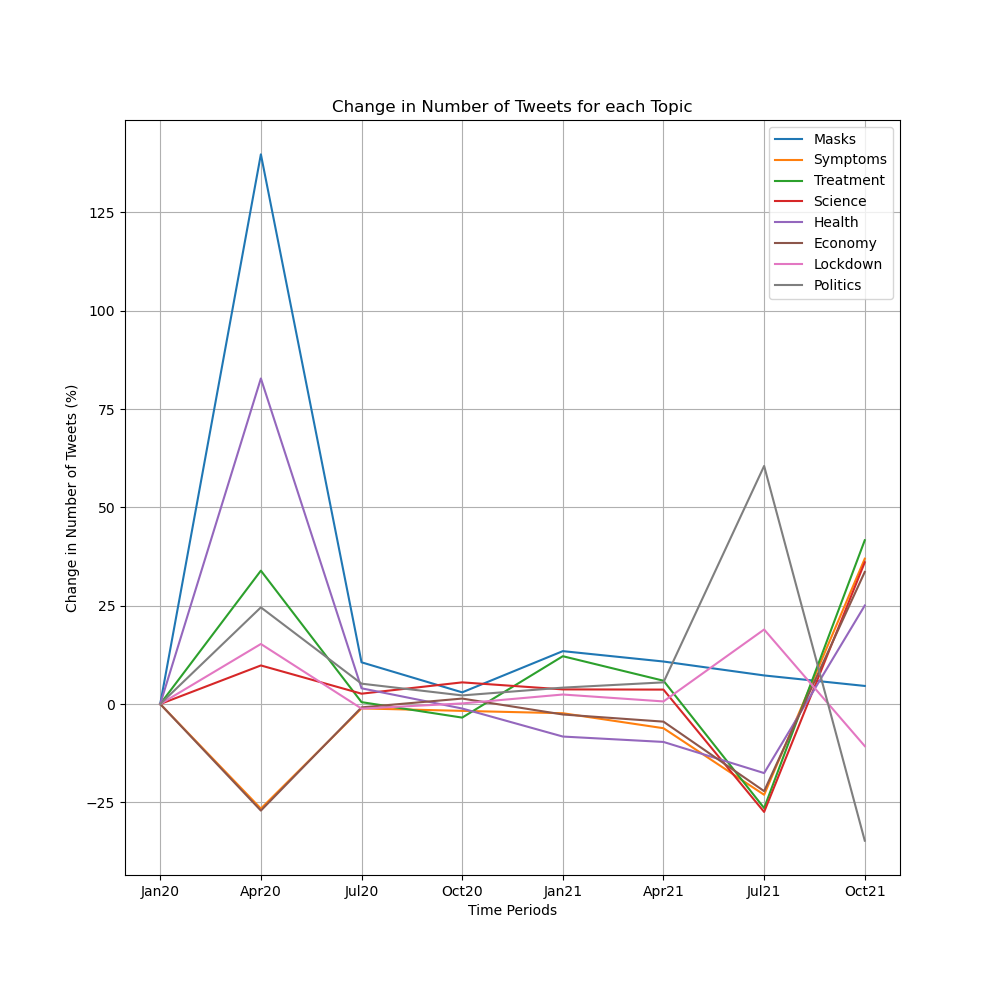
\includegraphics[width=1.0\linewidth]{images/topicNum.png}
    \caption{Change in Number of Tweets per Topic Over Time}
\end{figure}

Since then there haven't been any significant ups and downs until April 2021. Considering that the 1M tweets we're using were randomly sampled from around 300M English Covid-19 tweets, this is quite interesting to see. One thing to note is that health is getting fewer tweets since April 2020. Either there hasn't been much to talk about, doubtful since there have been a lot of developments regarding the virus with its variants and vaccines (\cite{covidhist}) or Twitter is not a platform where health discussions take place.

July 2021 is when we see a rather significant shift. Politics gains a major boost in the number of tweets while the topics other than lockdown all fall. This is likely due to the various legislation passed by governments across the world to lift Covid-19 restrictions and bring things back to normalcy. Lastly, in October, all of the medical/technical topics gain a rise in popularity with a 25\% increase from July.

After seeing how topics have trended over 2 years, let's see how this impacts the amount of misinformation. In figure 5.2 we can see that the ration of misinformation decreases for all of the topics, particularly health which saw a over a 30\% decrease due to the 75\% increase in the number of tweets.

\begin{figure}[h]
    \centering
    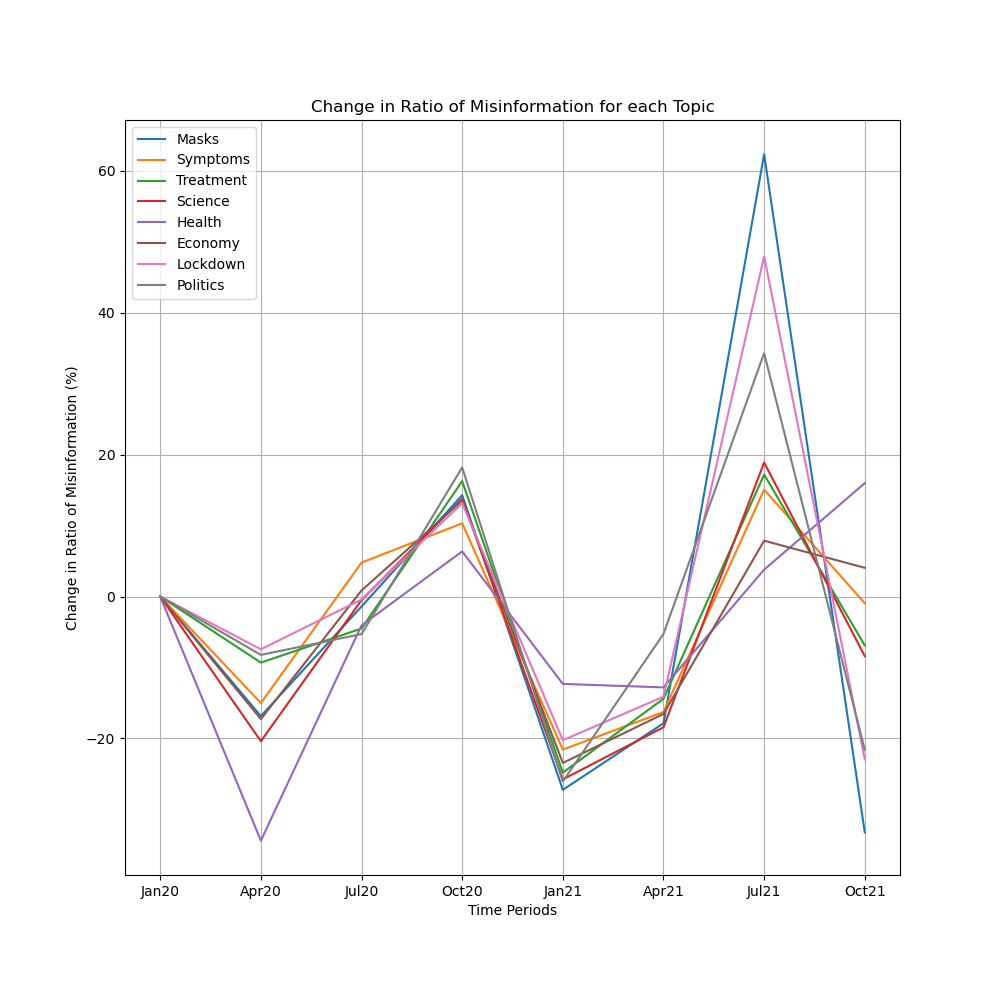
\includegraphics[width=1.0\linewidth]{images/topicMisinfo.png}
    \caption{Change in Ratio of Misinformation per Topic Over Time}
\end{figure}

However, this downward trend does not continue as shown by July and October 2020 when the ratio of misinformation continues to increase. For this period of time, the number of tweets increases for some topics and decreases for others so there's no conclusive evidence that suggests that an increase in the quantity of information leads to less misinformation. This is especially true for the next periods where we see in figure 5.1 that there are small ups and downs for all the topics, accompanied by a 20\%+ decrease in the misinformation ratio for January 2021 with a slight increase for April.

Moving on to July, we see a sharp rise in misinformation across all the topics with masks having a staggering 60\% increase from the previous period which does correspond to the decline in the number of tweets per topic. However, politics saw a rise in tweet count but despite that, there is a 30\% increase in misinformation. This might be more due to the divisive nature of politics leading to strong bias and propaganda more than anything else. Our final time periods show some improvement with misinformation falling or only increasing slightly for most of our topics however it should be noted that health has seen an increase in misinformation ever since April 2021 which isn't all that great considering the low number of tweets it has.

From our analysis of the misinformation per topic in each period, we can see while there is some correlation between data quantity and misinformation, at points a rise in the number of tweets led to a fall in misinformation and vice versa, there was enough variation to make it so we cannot make a proper conclusion without having an overall look at the data (section 5.4).

\section{Sentiment Analysis}

In this section, we will look at the correlation between the sentiments of each topic and the misinformation they contain. For Masks, in figure \ref{fig:masksen} and table \ref{tab:masksen} we can see that negative sentiment has a moderate positive correlation with an increase in misinformation whereas positive sentiment has a moderate negative correlation while neutral has almost no correlation.

\begin{table}[h]
\begin{minipage}[c]{0.30\linewidth}
\centering
\begin{tabular}{@{}ll@{}}
\toprule
Sentiment & Pearson Correlation Coefficient \\ \midrule
Positive  & \multicolumn{1}{c}{-0.522}      \\
Negative  & \multicolumn{1}{c}{0.508}       \\
Neutral   & \multicolumn{1}{c}{0.027}       \\ \bottomrule
\end{tabular}
\caption{Pearson Correlation Coefficients for Masks Sentiment}
\label{tab:masksen}
\end{minipage}\hfill
\begin{minipage}[c]{0.55\linewidth}
\centering
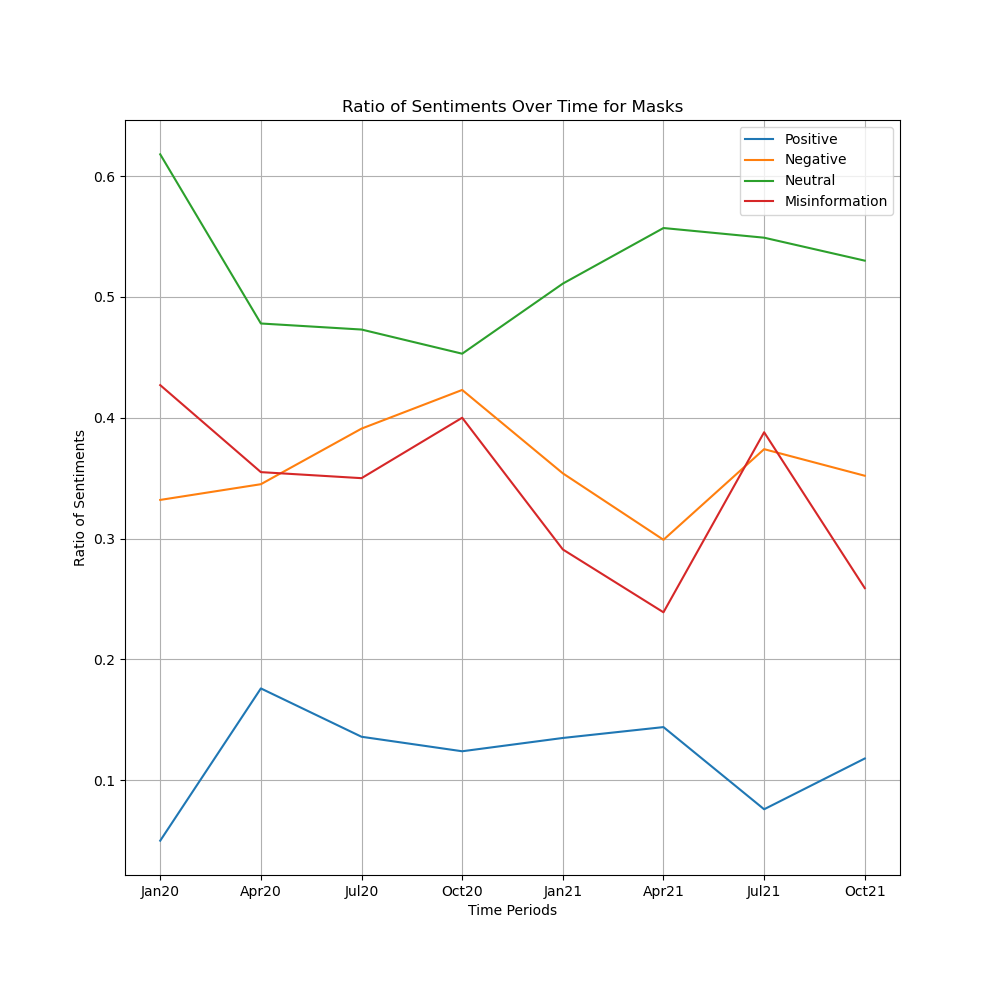
\includegraphics[width=\textwidth]{images/MasksSentiment.png}
\captionof{figure}{Ratios of Sentiment and Misinformation for Masks}
\label{fig:masksen}
\end{minipage}
\end{table}

For Symptoms, in figure \ref{fig:sympsen} and table \ref{tab:sympsen} just like with Masks, there is a strong positive and negative correlation for negative and positive sentiments respectively with neutral having a very weak negative correlation. So far we can see that negative sentiment contributes more to misinformation while positive sentiment is the opposite.


\begin{table}[h]
\begin{minipage}[c]{\linewidth}
\centering
\begin{tabular}{@{}ll@{}}
\toprule
Sentiment & Pearson Correlation Coefficient \\ \midrule
Positive  & \multicolumn{1}{c}{-0.698}      \\
Negative  & \multicolumn{1}{c}{0.698}       \\
Neutral   & \multicolumn{1}{c}{-0.135}       \\ \bottomrule
\end{tabular}
\caption{Pearson Correlation Coefficients for Symptoms Sentiment}
\label{tab:sympsen}
\end{minipage}\hfill
\end{table}

For the topic Treatment, figure \ref{fig:treatsen} and table \ref{tab:treatsen} show that negative sentiment has a moderate positive correlation, positive sentiment has a moderate negative correlation, and neutral sentiment has almost no correlation with an increase in misinformation. The trend from earlier continues.

\begin{table}[H]
\begin{minipage}[c]{\linewidth}
\centering
\begin{tabular}{@{}ll@{}}
\toprule
Sentiment & Pearson Correlation Coefficient \\ \midrule
Positive  & \multicolumn{1}{c}{-0.454}      \\
Negative  & \multicolumn{1}{c}{0.583}       \\
Neutral   & \multicolumn{1}{c}{-0.004}       \\ \bottomrule
\end{tabular}
\caption{Pearson Correlation Coefficients for Treatment Sentiment}
\label{tab:treatsen}
\end{minipage}\hfill
\end{table}

In figure \ref{fig:scisen} and table \ref{fig:scisen} a strong positive correlation is observed for negative sentiment in Science as well as a moderate negative correlation for positive sentiment and a very weak positive correlation for neutral sentiment. Thus far half of our topics of interest have shown high correlation coefficients for negative sentiment so it's likely that it's a characteristic of misinformation.

\begin{table}[h]
\begin{minipage}[c]{\linewidth}
\centering
\begin{tabular}{@{}ll@{}}
\toprule
Sentiment & Pearson Correlation Coefficient \\ \midrule
Positive  & \multicolumn{1}{c}{-0.568}      \\
Negative  & \multicolumn{1}{c}{0.631}       \\
Neutral   & \multicolumn{1}{c}{0.024}       \\ \bottomrule
\end{tabular}
\caption{Pearson Correlation Coefficients for Science Sentiment}
\label{tab:scisen}
\end{minipage}\hfill

\end{table}

Health is where we see our first departure from the norm. Figure \ref{fig:healthsen} and table \ref{fig:healthsen} show that positive sentiment has a very strong negative correlation, negative sentiment has a very weak positive correlation, and neutral sentiment has a strong positive correlation to misinformation. So far this is a first for us since it shows that it's not always the case that misinformation is characterised by negative sentiment.

\begin{table}[H]
\begin{minipage}[c]{0.30\linewidth}
\centering
\begin{tabular}{@{}ll@{}}
\toprule
Sentiment & Pearson Correlation Coefficient \\ \midrule
Positive  & \multicolumn{1}{c}{-0.881}      \\
Negative  & \multicolumn{1}{c}{0.027}       \\
Neutral   & \multicolumn{1}{c}{0.708}       \\ \bottomrule
\end{tabular}
\caption{Pearson Correlation Coefficients for Health Sentiment}
\label{tab:healthsen}
\end{minipage}\hfill
\begin{minipage}[c]{0.55\linewidth}
\centering
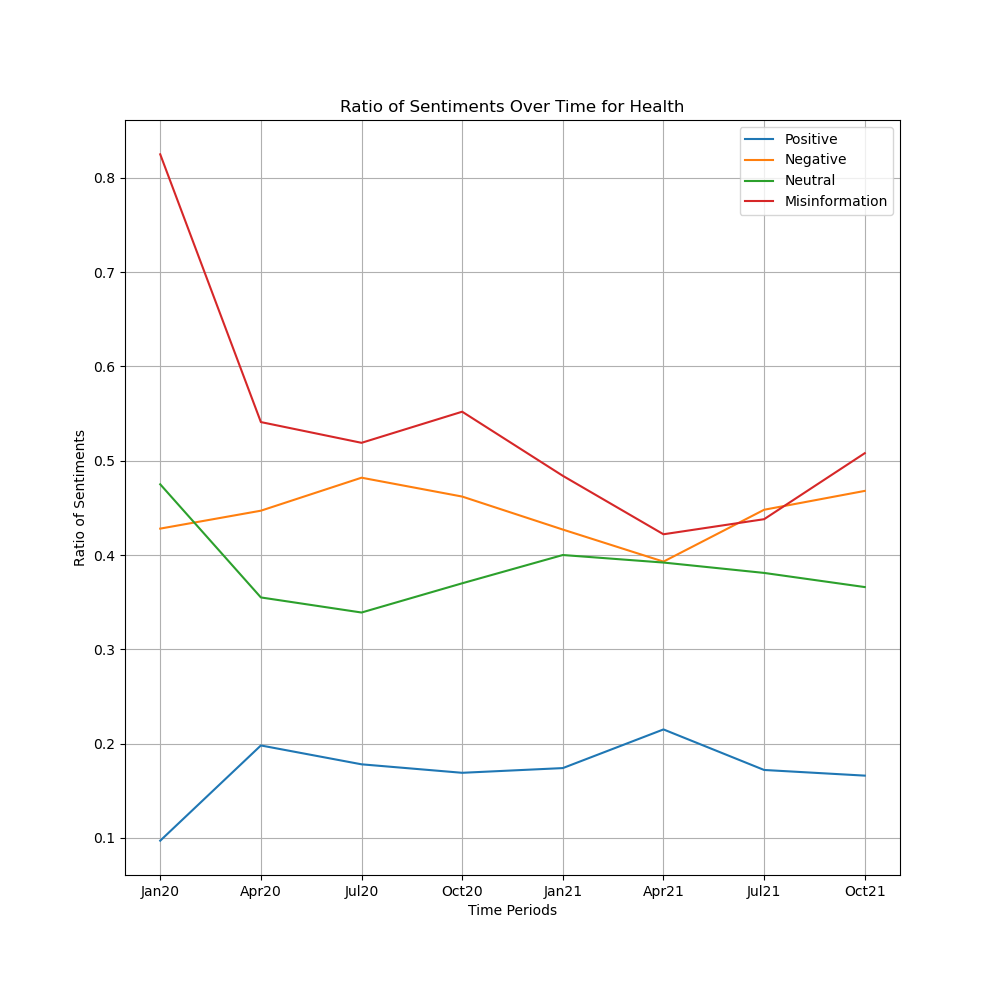
\includegraphics[width=\textwidth]{images/HealthSentiment.png}
\captionof{figure}{Ratios of Sentiment and Misinformation for Health}
\label{fig:healthsen}
\end{minipage}
\end{table}

We return to earlier results with Economy. In figure \ref{fig:ecosen} and table \ref{tab:ecosen} we can see that negative sentiment has a moderate positive correlation while positive and neutral sentiment have very strong and very weak correlations respectively.

\begin{table}[h]
\begin{minipage}[c]{\linewidth}
\centering
\begin{tabular}{@{}ll@{}}
\toprule
Sentiment & Pearson Correlation Coefficient \\ \midrule
Positive  & \multicolumn{1}{c}{-0.611}      \\
Negative  & \multicolumn{1}{c}{0.555}       \\
Neutral   & \multicolumn{1}{c}{-0.031}       \\ \bottomrule
\end{tabular}
\caption{Pearson Correlation Coefficients for Economy Sentiment}
\label{tab:ecosen}
\end{minipage}\hfill

\end{table}

We don't see any significant change for Lockdown in figure \ref{fig:locksen} and table \ref{tab:locksen}. Negative sentiment has a moderate positive correlation, positive sentiment has a strong negative correlation and finally, natural sentiment has a very weak negative correlation.

\begin{table}[H]
\begin{minipage}[c]{\linewidth}
\centering
\begin{tabular}{@{}ll@{}}
\toprule
Sentiment & Pearson Correlation Coefficient \\ \midrule
Positive  & \multicolumn{1}{c}{-0.618}      \\
Negative  & \multicolumn{1}{c}{0.583}       \\
Neutral   & \multicolumn{1}{c}{-0.054}       \\ \bottomrule
\end{tabular}
\caption{Pearson Correlation Coefficients for Lockdown Sentiment}
\label{tab:locksen}
\end{minipage}\hfill

\end{table}

Lastly, for Politics, in figure \ref{fig:polsen} and table \ref{tab:polsen} we observe that both positive and negative sentiment have a moderate negative and positive correlation respectively whereas neutral sentiment is hardly correlated to misinformation.

\begin{table}[h]
\begin{minipage}[c]{\linewidth}
\centering
\begin{tabular}{@{}ll@{}}
\toprule
Sentiment & Pearson Correlation Coefficient \\ \midrule
Positive  & \multicolumn{1}{c}{-0.509}      \\
Negative  & \multicolumn{1}{c}{0.405}       \\
Neutral   & \multicolumn{1}{c}{0.001}       \\ \bottomrule
\end{tabular}
\caption{Pearson Correlation Coefficients for Politics Sentiment}
\label{tab:polsen}
\end{minipage}\hfill

\end{table}

From our topics, we saw a moderate to strong positive correlation for negative sentiment in seven of them which means we can confidently say negative sentiment is a characteristic of misinformation.

\section{Emotion Analysis}
In this section, we will look at the correlation between the emotions in each topic and misinformation. Figure \ref{fig:maskemo} and table \ref{tab:maskemo} show that we have a strong positive correlation for surprise, moderate positive correlations for anger and disgust, and weak negative correlations for joy, sadness, and fear. 

\begin{table}[H]
\begin{minipage}[c]{0.30\linewidth}
\centering
\begin{tabular}{@{}lc@{}}
\toprule
Emotion  & \multicolumn{1}{l}{Pearson Correlation Coefficient} \\ \midrule
Joy      & -0.237                                              \\
Sadness  & -0.410                                              \\
Anger    & 0.574                                               \\
Surprise & 0.678                                               \\
Disgust  & 0.591                                               \\
Fear     & -0.373                                              \\ \bottomrule
\end{tabular}
\caption{Pearson Correlation Coefficients for Masks Emotions}
\label{tab:maskemo}
\end{minipage}\hfill
\begin{minipage}[c]{0.55\linewidth}
\centering
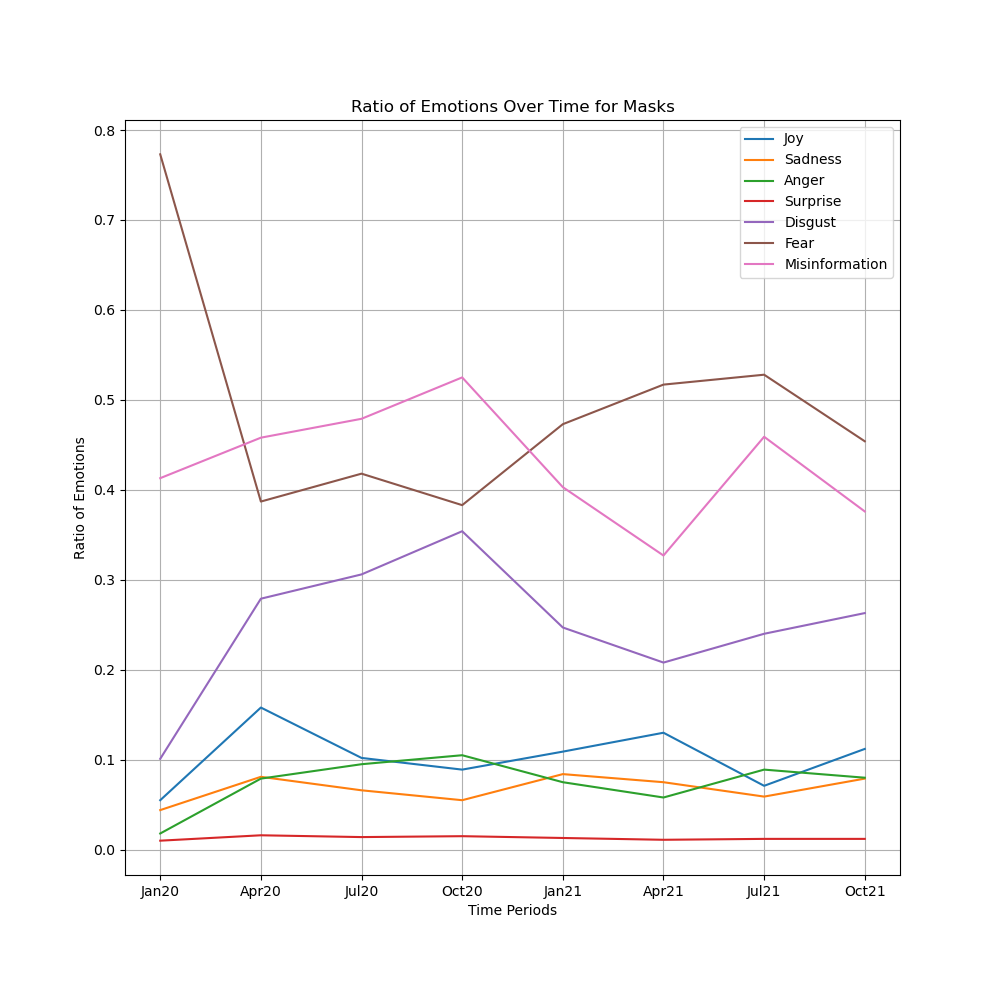
\includegraphics[width=\textwidth]{images/MasksEmotion.png}
\captionof{figure}{Ratios of Emotions and Misinformation for Masks}
\label{fig:maskemo}
\end{minipage}
\end{table}

For Symptoms, we can see moderate positive correlations for anger and disgust in figure \ref{fig:sympemo} and table \ref{tab:sympemo} alongside weak correlation for joy, sadness, and fear, and a very weak negative correlation for a surprise.

\begin{table}[h]
\begin{minipage}[c]{\linewidth}
\centering
\begin{tabular}{@{}lc@{}}
\toprule
Emotion  & \multicolumn{1}{l}{Pearson Correlation Coefficient} \\ \midrule
Joy      & -0.362                                              \\
Sadness  & -0.364                                              \\
Anger    & 0.466                                              \\
Surprise & -0.012                                               \\
Disgust  & 0.561                                               \\
Fear     & -0.283                                              \\ \bottomrule
\end{tabular}
\caption{Pearson Correlation Coefficients for Symptoms Emotions}
\label{tab:sympemo}
\end{minipage}\hfill

\end{table}

For Treatment, we see in figure \ref{fig:treatemo} and table \ref{tab:treatemo} that other than fear, which has a strong negative correlation, the others all have positive correlations ranging from very weak (joy), weak (sadness), moderate (anger, surprise) and strong (disgust). It's interesting how almost all of the emotions contribute to increasing misinformation about the topic.

\begin{table}[h]
\begin{minipage}[c]{\linewidth}
\centering
\begin{tabular}{@{}lc@{}}
\toprule
Emotion  & \multicolumn{1}{l}{Pearson Correlation Coefficient} \\ \midrule
Joy      & 0.147                                              \\
Sadness  & 0.246                                              \\
Anger    & 0.561                                               \\
Surprise & 0.406                                               \\
Disgust  & 0.644                                               \\
Fear     & -0.542                                              \\ \bottomrule
\end{tabular}
\caption{Pearson Correlation Coefficients for Treatment Emotions}
\label{tab:treatemo}
\end{minipage}\hfill

\end{table}

In figure \ref{fig:sciemo} and table \ref{tab:sciemo} for Science, we can see weak negative correlations for joy and sadness, moderate positive correlations for anger and disgust, and very weak negative and positive correlations for fear and surprise respectively.

\begin{table}[H]
\begin{minipage}[c]{\linewidth}
\centering
\begin{tabular}{@{}lc@{}}
\toprule
Emotion  & \multicolumn{1}{l}{Pearson Correlation Coefficient} \\ \midrule
Joy      & -0.340                                              \\
Sadness  & -0.324                                              \\
Anger    & 0.424                                               \\
Surprise & 0.205                                               \\
Disgust  & 0.423                                               \\
Fear     & -0.133                                              \\ \bottomrule
\end{tabular}
\caption{Pearson Correlation Coefficients for Science Emotions}
\label{tab:sciemo}
\end{minipage}\hfill

\end{table}

For Health in figure \ref{fig:healthemo} and table \ref{tab:healthemo} there is a very weak and strong positive correlation for sadness and fear respectively, a weak negative correlation for disgust, a moderate negative correlation for anger and surprise, and very strong negative correlation for joy. In previous topics, anger, surprise, and disgust had positive correlations while fear had a negative one but here it is the opposite like for sentiment analysis.

\begin{table}[H]
\begin{minipage}[c]{0.30\linewidth}
\centering
\begin{tabular}{@{}lc@{}}
\toprule
Emotion  & \multicolumn{1}{l}{Pearson Correlation Coefficient} \\ \midrule
Joy      & -0.900                                              \\
Sadness  & 0.181                                              \\
Anger    & -0.458                                               \\
Surprise & -0.511                                               \\
Disgust  & -0.223                                               \\
Fear     & 0.758                                              \\ \bottomrule
\end{tabular}
\caption{Pearson Correlation Coefficients for Health Emotions}
\label{tab:healthemo}
\end{minipage}\hfill
\begin{minipage}[c]{0.55\linewidth}
\centering
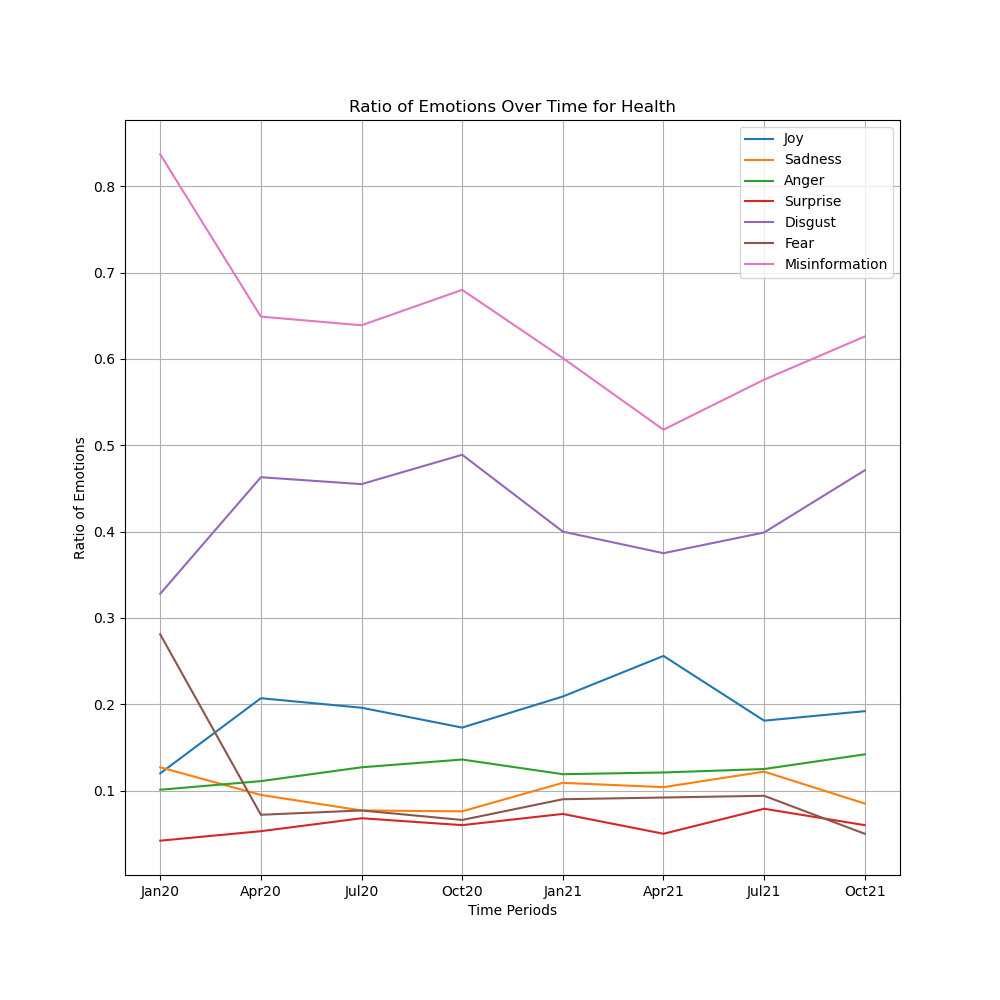
\includegraphics[width=\textwidth]{images/HealthEmotion.png}
\captionof{figure}{Ratios of Emotions and Misinformation for Health}
\label{fig:healthemo}
\end{minipage}
\end{table}

Economy has a moderate positive correlation for anger and disgust in figure \ref{fig:ecoemo} and table \ref{tab:ecoemo} as well as a very weak positive correlation for surprise. Joy and fear have weak negative correlations and sadness has a moderate negative correlation.

\begin{table}[h]
\begin{minipage}[c]{\linewidth}
\centering
\begin{tabular}{@{}lc@{}}
\toprule
Emotion  & \multicolumn{1}{l}{Pearson Correlation Coefficient} \\ \midrule
Joy      & -0.317                                              \\
Sadness  & -0.568                                              \\
Anger    & 0.402                                               \\
Surprise & 0.178                                               \\
Disgust  & 0.468                                               \\
Fear     & -0.230                                              \\ \bottomrule
\end{tabular}
\caption{Pearson Correlation Coefficients for Economy Emotions}
\label{tab:ecoemo}
\end{minipage}\hfill

\end{table}

The topic Lockdown has a very weak negative correlations for joy and sadness in figure \ref{fig:lockemo} and table \ref{tab:lockemo} and strong negative correlation with fear. There's a weak and strong positive correlation for surprise and anger respectively, and finally there is a very strong correlation for disgust.

\begin{table}[h]
\begin{minipage}[c]{\linewidth}
\centering
\begin{tabular}{@{}lc@{}}
\toprule
Emotion  & \multicolumn{1}{l}{Pearson Correlation Coefficient} \\ \midrule
Joy      & -0.065                                              \\
Sadness  & -0.046                                              \\
Anger    & 0.761                                               \\
Surprise & 0.296                                               \\
Disgust  & 0.802                                               \\
Fear     & -0.655                                              \\ \bottomrule
\end{tabular}
\caption{Pearson Correlation Coefficients for Lockdown Emotions}
\label{tab:lockemo}
\end{minipage}\hfill

\end{table}

Finally for Politics, in figure \ref{fig:polemo} and table \ref{tab:polemo} we observe a strong positive correlation for the emotions of anger and disgust, a weak positive correlation for surprise, very weak and weak negative correlations for joy and sadness, and a strong negative correlation for fear.

\begin{table}[H]
\begin{minipage}[c]{\linewidth}
\centering
\begin{tabular}{@{}lc@{}}
\toprule
Emotion  & \multicolumn{1}{l}{Pearson Correlation Coefficient} \\ \midrule
Joy      & -0.038                                              \\
Sadness  & -0.239                                              \\
Anger    & 0.696                                               \\
Surprise & 0.267                                               \\
Disgust  & 0.713                                               \\
Fear     & -0.587                                              \\ \bottomrule
\end{tabular}
\caption{Pearson Correlation Coefficients for Politics Emotions}
\label{tab:polemo}
\end{minipage}\hfill

\end{table}

From our findings, we see a moderate to strong positive correlation for anger and disgust and a weak to moderate correlation for surprise for most of the topics so we can safely see these three emotions are characteristics of misinformation.

\section{Overall Result}
In this section, we'll consolidate our findings to answer our research question and prove the hypothesis. In sections 5.2 and 5.3 we concluded that negative sentiment, anger, surprise, and disgust are all characteristics of misinformation by looking at the individual topics. After finding the mean of the coefficients, we see in tables \ref{tab:avgsen} and \ref{tab:avgemo} that negative sentiment, anger, and disgust all have a moderate positive correlation to misinformation so they indeed are characteristics of it. Surprise has a very weak positive correlation so it can't be called a proper characteristic. 

\begin{table}[H]
\begin{minipage}[c]{0.45\linewidth}
\centering
\begin{tabular}{@{}lc@{}}
\toprule
Sentiment  & \multicolumn{1}{l}{Pearson Correlation Coefficient} \\ \midrule
Positive      & -0.608                                              \\
Negative  & 0.499                                              \\
Neutral     & 0.067                                              \\ \bottomrule
\end{tabular}
\caption{Average Pearson Correlation Coefficients for Sentiment}
\label{tab:avgsen}
\end{minipage}\hfill
\begin{minipage}[c]{0.45\linewidth}
\centering
\begin{tabular}{@{}lc@{}}
\toprule
Emotion  & \multicolumn{1}{l}{Pearson Correlation Coefficient} \\ \midrule
Joy      & -0.264                                              \\
Sadness  & -0.190                                              \\
Anger    & 0.428                                               \\
Surprise & 0.188                                               \\
Disgust  & 0.497                                               \\
Fear     & -0.256                                              \\ \bottomrule
\end{tabular}
\caption{Average Pearson Correlation Coefficients for Emotions}
\label{tab:avgemo}
\end{minipage}
\end{table}

From what has been observed, misinformation increases or decreases depending on the period but in general there seems to be a downward trend. In figure \ref{fig:overall} we can see that in the beginning the overall ratio of misinformation for January 2020 was over 0.50 but it gradually fell to just under 0.40 in October 2021. This shows clearly that without us having to do anything, misinformation naturally decreases over time as the quantity of information available increases. This proves our hypothesis.

And now that we know the characteristics of misinformation, we filtered out tweets with a combination of them from the dataset and the cumulative misinformation ratio of the filtered dataset was plotted in \ref{fig:overall}, showing there's a drastic reduction in misinformation with around a 10\% decrease in January 2020, down to a ration of 0.25 in October 2021. With these results we also answer our research question:

\vspace{0.4cm}
\begin{center}
    "To what extent does the passage of time affect the quantity of misinformation floating online? And what are the identifying characteristics of such information?"
\end{center}
\vspace{0.4cm}

Other than emotions and sentiment, we'd also like to know if any topics correlate to an increase in misinformation. Based on table \ref{tab:avgtopic} however, that does not seem to be a case. Of our selected topics, only Treatment has a notable positive correlation but even then it's a weak correlation so there isn't any particular topic that contributes more to misinformation.


\begin{table}[H]
\centering
\resizebox{\textwidth}{!}{%
\begin{tabular}{@{}lcccccccc@{}}
          & \multicolumn{1}{l}{Masks} & \multicolumn{1}{l}{Symptoms} & \multicolumn{1}{l}{Treatment} & \multicolumn{1}{l}{Science} & \multicolumn{1}{l}{Health} & \multicolumn{1}{l}{Economy} & \multicolumn{1}{l}{Lockdown} & \multicolumn{1}{l}{Politics} \\ \midrule
Sentiment & 0.004                     & -0.045                       & 0.042                         & 0.029                       & -0.049                     & -0.029                      & -0.030                       & -0.034                       \\
Emotion   & 0.137                     & 0.001                        & 0.244                         & 0.042                       & -0.192                     & -0.011                      & 0.182                        & 0.135                       \\ \bottomrule
\end{tabular}%
}
\caption{Average Pearson Correlation Coefficients for Topics}
\label{tab:avgtopic}
\end{table}

\begin{figure}[H]
    \centering
    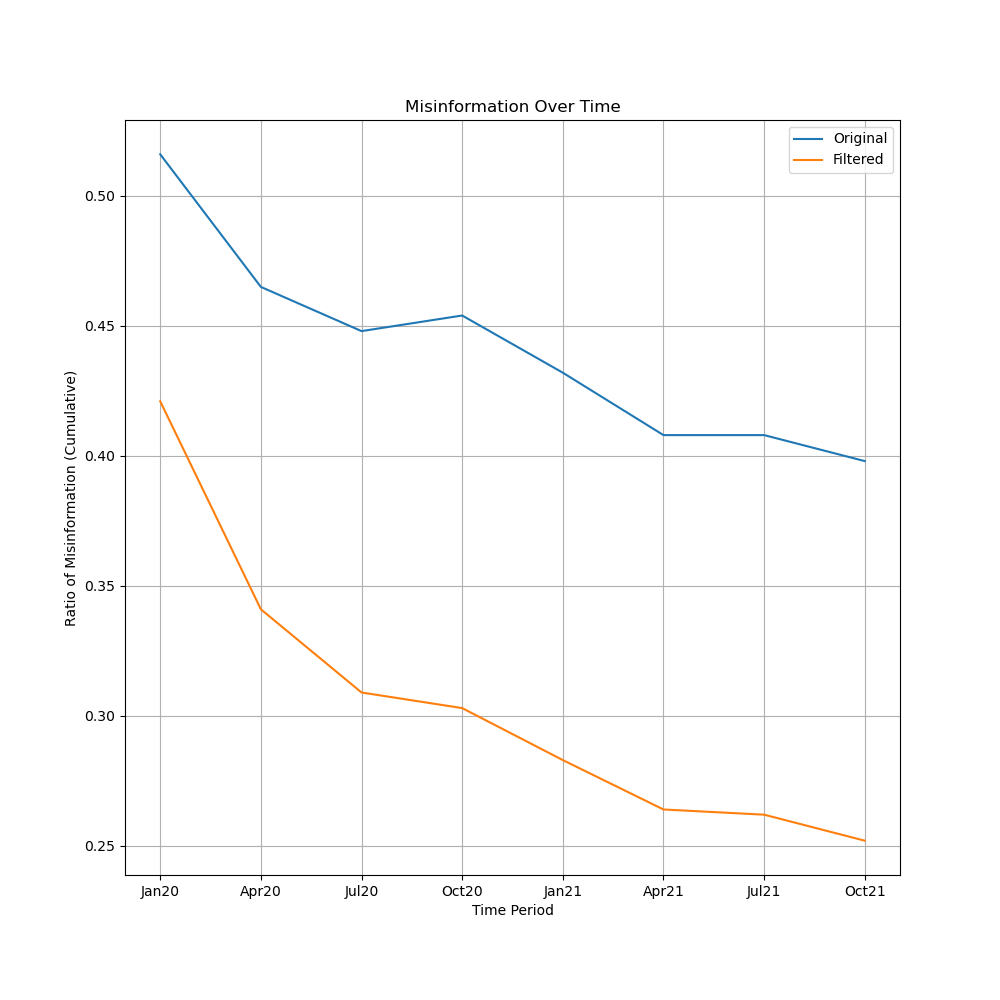
\includegraphics[width=1.0\linewidth]{images/misinfoPlotv2.png}
    \caption{Cumulative Misinformation Over Time}
    \label{fig:overall}
\end{figure}

With these findings, we can do a lot to reduce the quantity of health misinformation, and fake news in general, that people can come across. One application is to create a search engine filter that scans results for negative sentiment and the underlying emotions of anger and disgust. These results can then be filtered out so that they don't appear at all or weights can be applied to make them less likely to show up.

To implement this we will need to train a classification model which actively flags results with these characteristics. A BERT-large model like Covid-Twitter-Bert-v2 would be good due to the complexity and performance as witnessed earlier on in section 4.2. We can combine this with a search engine or basic web crawler and deploy it in the real world to gather user feedback and use it to further finetune and improve the model to the point it can easily spot fake news and keep the general populace from being exposed to it.

%==================================================================================================================================
\chapter{Conclusion}    

\section{Summary}
To summarise everything we did over the course of this project, we first formulated a research question and hypothesis to form a foundation for the project. The two basically boiled down to us expecting misinformation to decrease over time. We then gathered around 1M tweets related to Covid-19 for eight time periods using a large dataset for scientific research. After hydrating the dataset (getting all the data related to the tweets via the tweet ids), we performed binary classification to label the tweets as either true or false using a BERT model specifically pre-trained to deal with Covid-19 tweets.

We then used Jaccard Similarity to group the tweets into fifteen topics and performed sentiment and emotion analysis on them to get the underlying sentiment and emotion for each tweet. Next, we calculated the Pearson Correlation Coefficient to find the characteristics of misinformation. This was visualised using tables and bar graphs and after analysing everything, we concluded that misinformation does naturally decrease over time and that by filtering out tweets with the following characteristics: negative sentiment, anger, and disgust; we would be able to reduce the misinformation even further.

Ultimately we were able to both prove the hypothesis and answer our research question to a great degree of success.

\section{Reflection}
I learned quite a lot by working on this project. My skills with data visualisation libraries and handling pandas dataframes has gone up considerably and I gained a lot of knowledge about various machine learning and nlp models. I also gained knowledge on AI in general by going over many papers related to the subject.

But there are a few things I am not satisfied with. For instance, I do not like how I had to default to using a statistical approach to group my tweets into topics instead on using clustering like I originally intended to. Were I able to do this project again, this is something I'd put extra emphasis on.

My binary classification could also use some work. I used a pre-existing dataset from earlier on in the pandemic to finetune a model which had most likely already seen those tweets which most likely resulted in a certain degree of overfitting. A more sensible approach would have been to expand that dataset with more recent tweets and manually annotate them so that the model would have some unseen data.

Overall though, I did the project to the best of my abilities and am satisfied with what I've achieved.

\section{Future work}
If given the opportunity to expand on this work and take it further, first of all, we would get data from other social media platforms like Reddit and Facebook and compare them with Twitter to see which source has the most misinformation. We would also use a proper clustering approach to group the data into topics and have a better, manually annotated training dataset combining tweets and Facebook and Reddit posts.

Then, we would also analyse the vocabulary used in misinformation to get a list of the most commonly used terms and use it in conjunction with the sentiment and emotion characteristics to develop a proper misinformation filter. For this, we'll train an NLP model like Bert-large and finetune it until the performance is satisfactory for our needs.

Finally, since the original proposal mentions ad-hoc search results, we would create a small database with a basic search engine and deploy it in the real world to simulate a proper search engine and have users input Covid-19 related queries to observe how much misinformation they stumble across. This user feedback will be used to catch misinformation characteristics we missed, and further improve our model.

%==================================================================================================================================
%
% 
%==================================================================================================================================
%  APPENDICES  

\begin{appendices}

\chapter{Sentiment Analysis Graphs}

\begin{figure}[H]
\begin{minipage}[c]{0.49\linewidth}
\centering
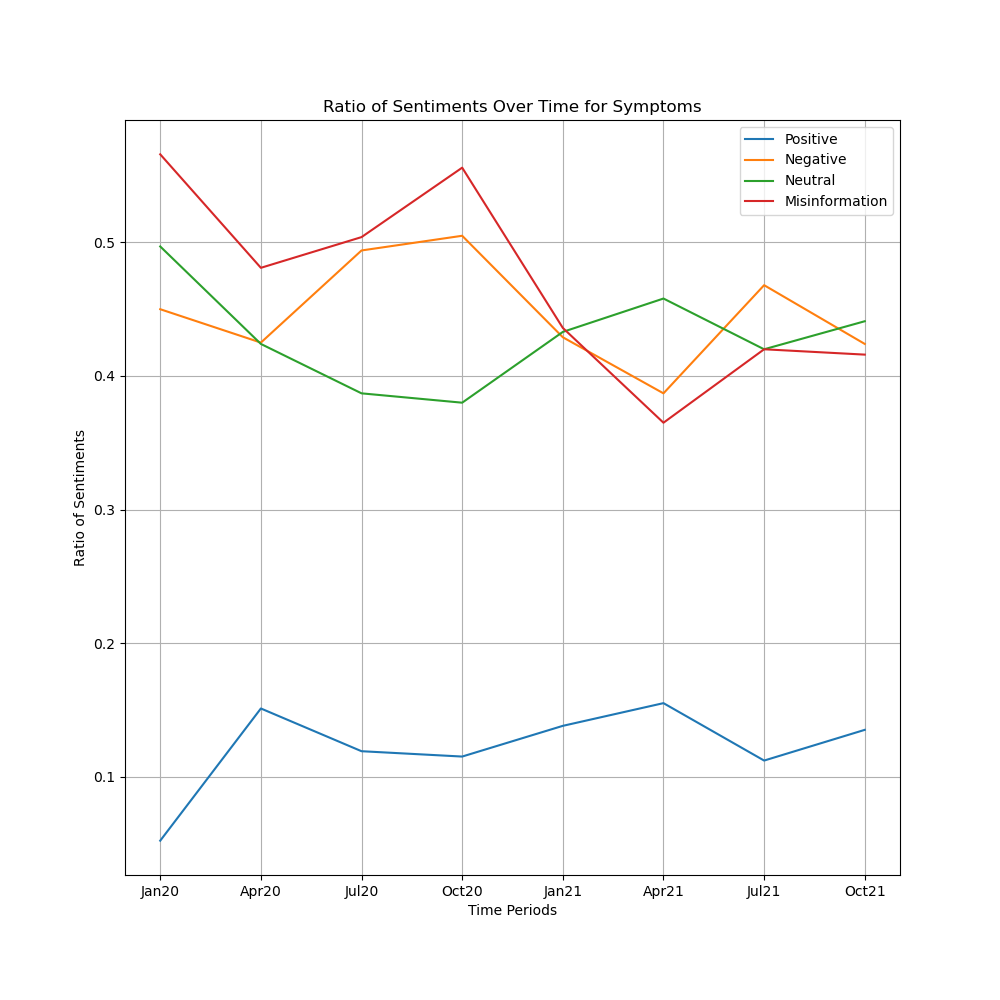
\includegraphics[width=\textwidth]{images/SymptomsSentiment.png}
\captionof{figure}{Ratios of Sentiment and Misinformation for Symptoms}
\label{fig:sympsen}
\end{minipage}\hfill
\begin{minipage}[c]{0.49\linewidth}
\centering
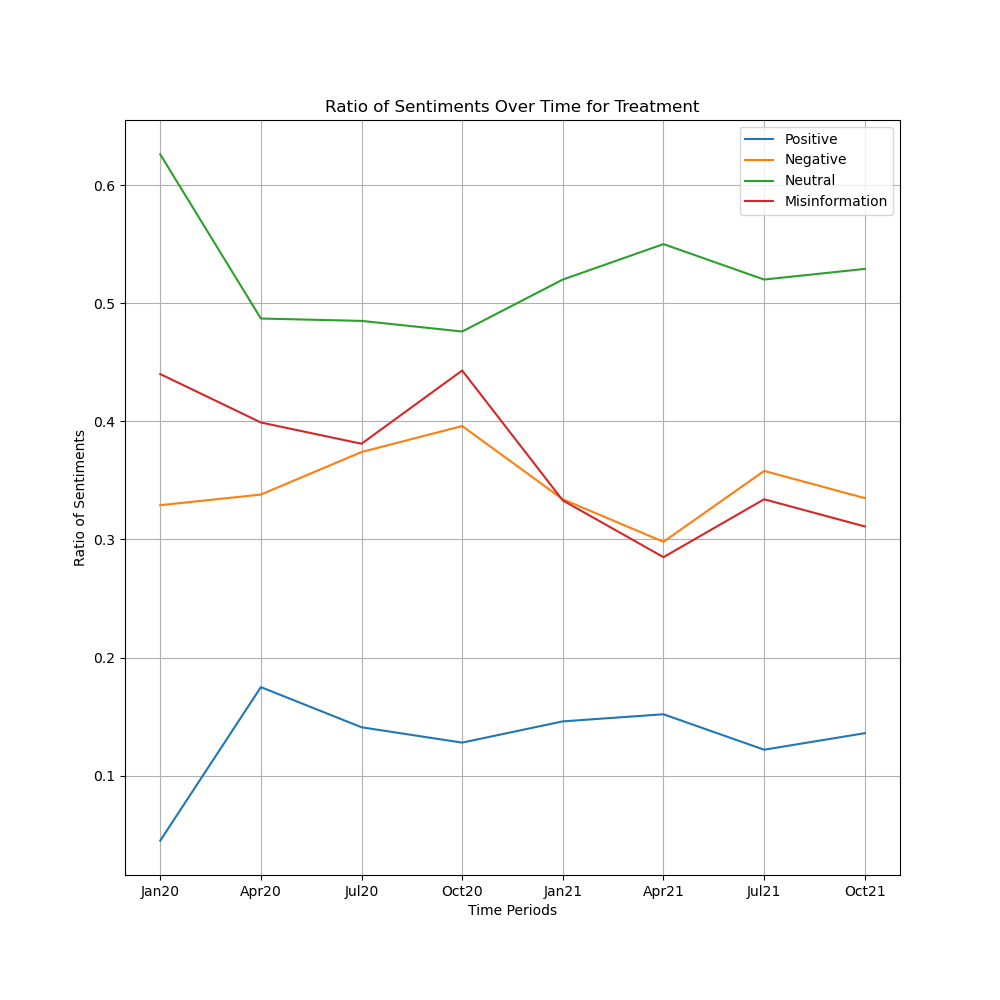
\includegraphics[width=\textwidth]{images/TreatmentSentiment.png}
\captionof{figure}{Ratios of Sentiment and Misinformation for Treatment}
\label{fig:treatsen}
\end{minipage}
\end{figure}

\begin{figure}[H]
\begin{minipage}[c]{0.49\linewidth}
\centering
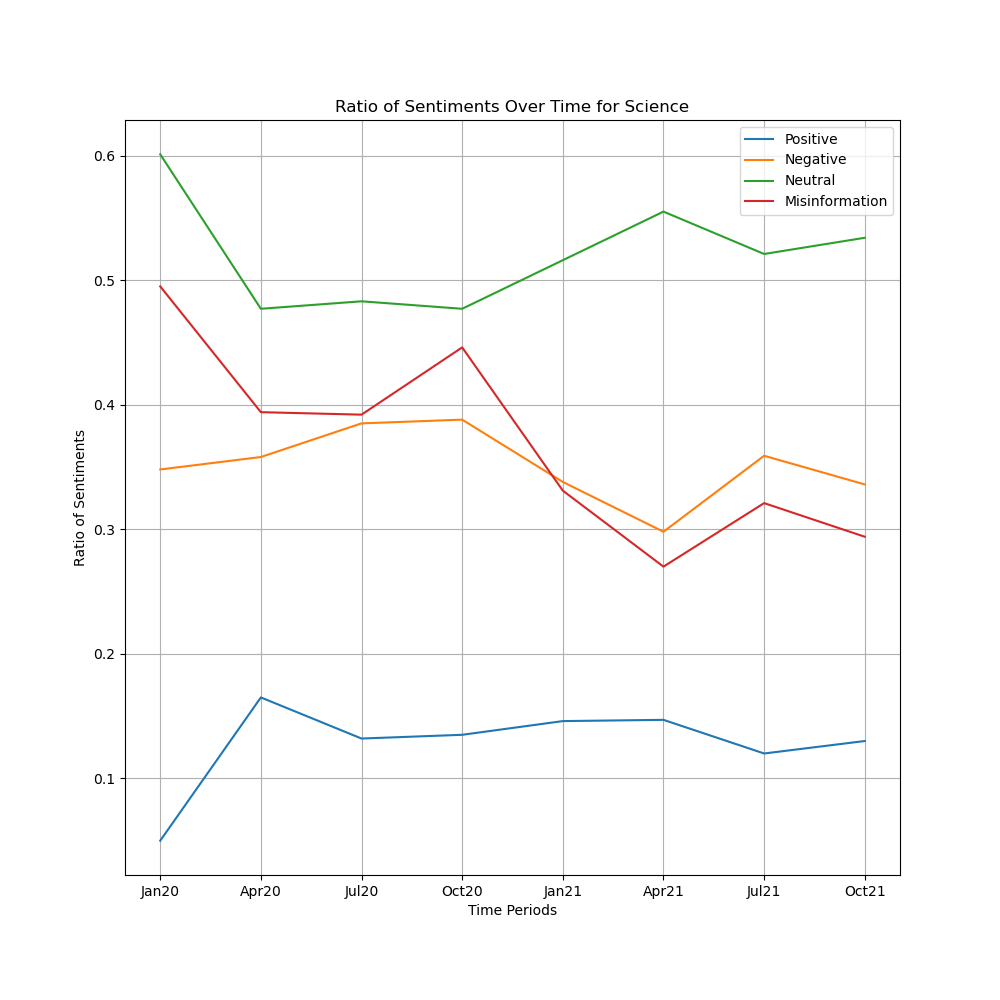
\includegraphics[width=\textwidth]{images/ScienceSentiment.png}
\captionof{figure}{Ratios of Sentiment and Misinformation for Science}
\label{fig:scisen}
\end{minipage}
\begin{minipage}[c]{0.49\linewidth}
\centering
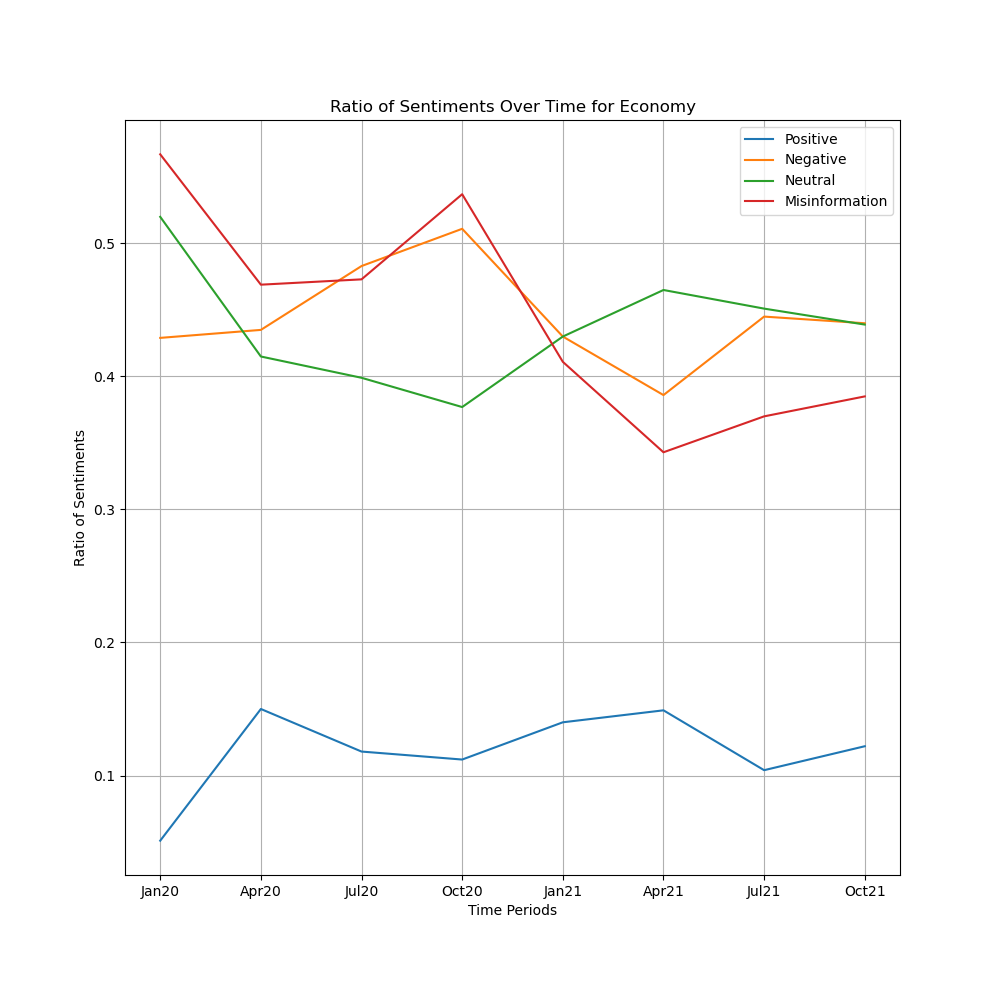
\includegraphics[width=\textwidth]{images/EconomySentiment.png}
\captionof{figure}{Ratios of Sentiment and Misinformation for Economy}
\label{fig:ecosen}
\end{minipage}
\end{figure}

\begin{figure}[H]
\begin{minipage}[c]{0.49\linewidth}
\centering
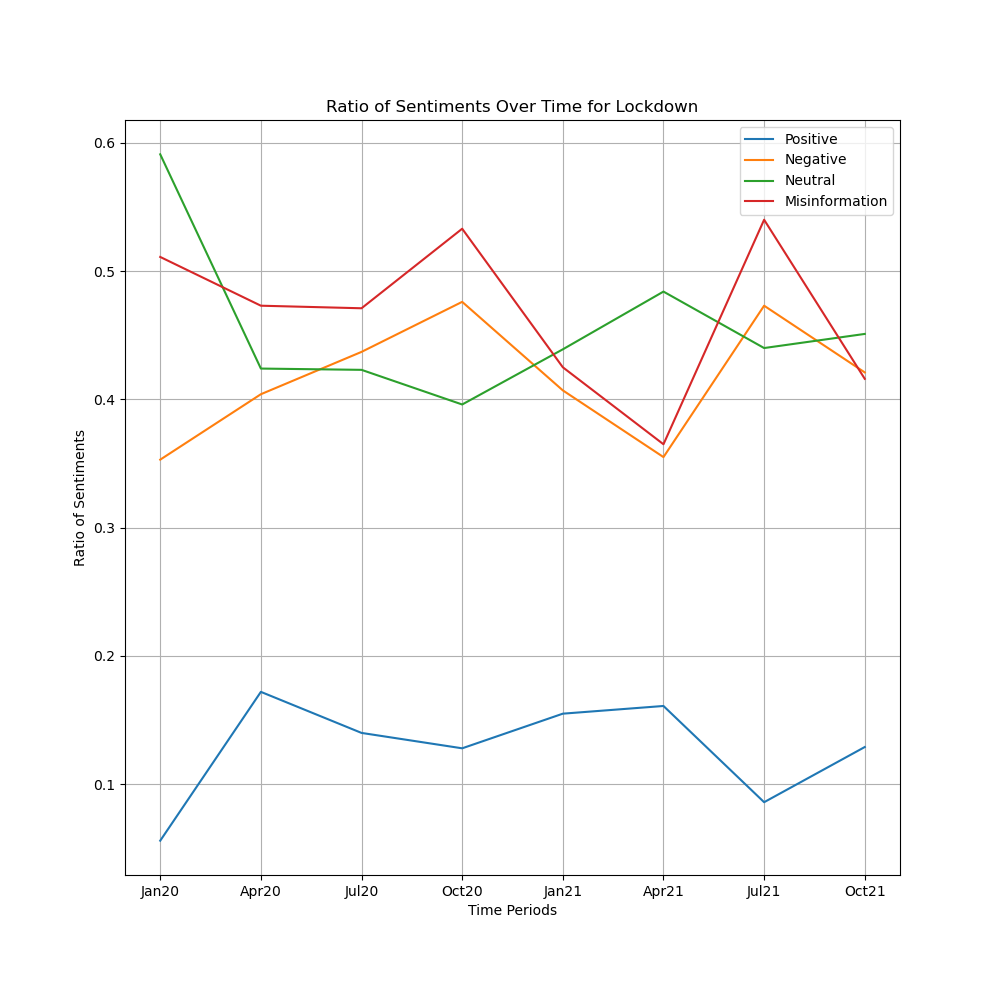
\includegraphics[width=\textwidth]{images/LockdownSentiment.png}
\captionof{figure}{Ratios of Sentiment and Misinformation for Lockdown}
\label{fig:locksen}
\end{minipage}
\begin{minipage}[c]{0.49\linewidth}
\centering
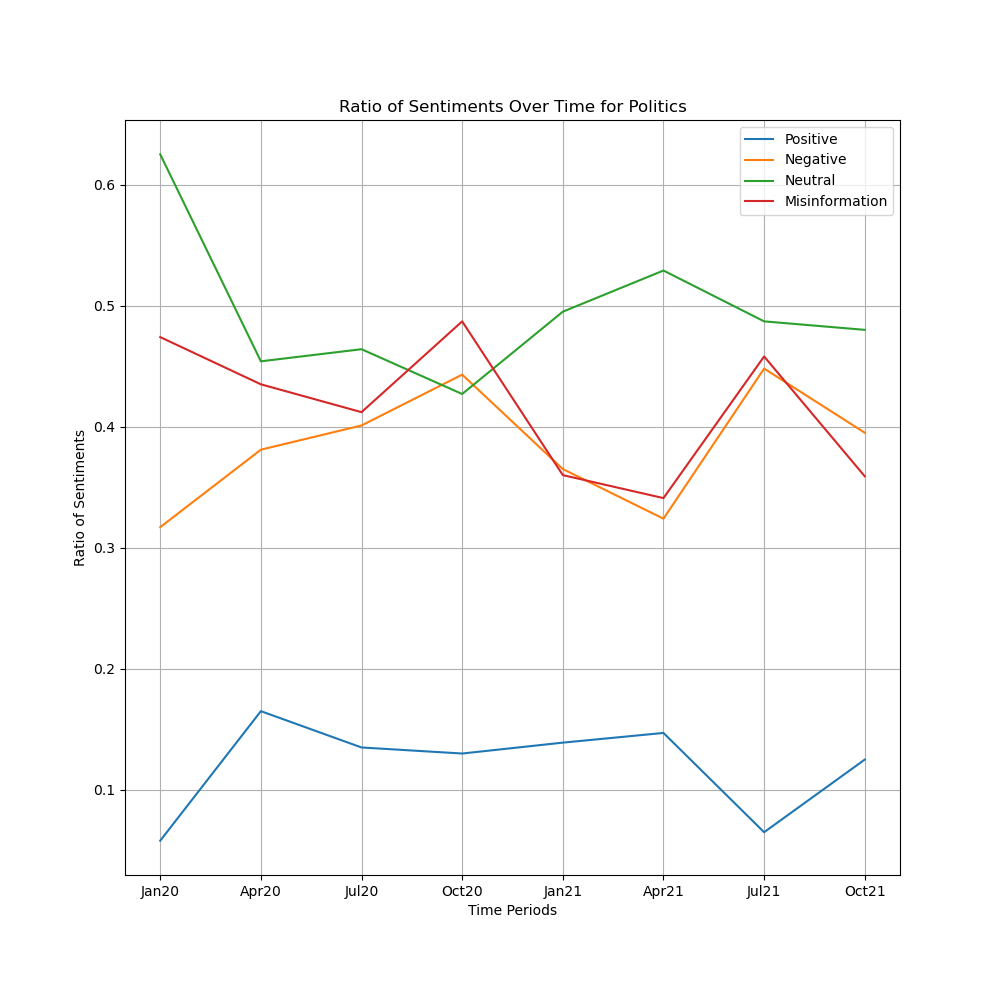
\includegraphics[width=\textwidth]{images/PoliticsSentiment.png}
\captionof{figure}{Ratios of Sentiment and Misinformation for Politics}
\label{fig:polsen}
\end{minipage}
\end{figure}

\chapter{Emotion Analysis Graphs}

\begin{figure}[H]
\begin{minipage}[c]{0.49\linewidth}
\centering
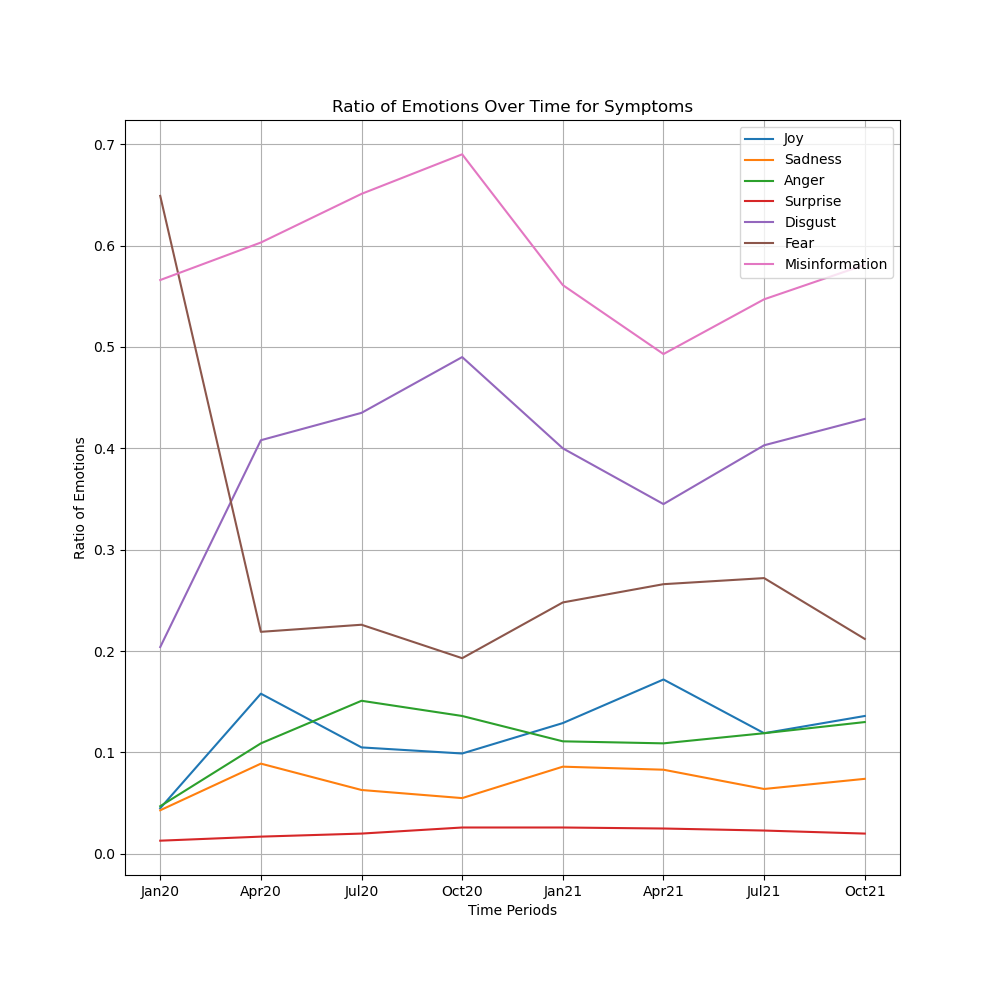
\includegraphics[width=\textwidth]{images/SymptomsEmotion.png}
\captionof{figure}{Ratios of Emotions and Misinformation for Symptoms}
\label{fig:sympemo}
\end{minipage}
\begin{minipage}[c]{0.49\linewidth}
\centering
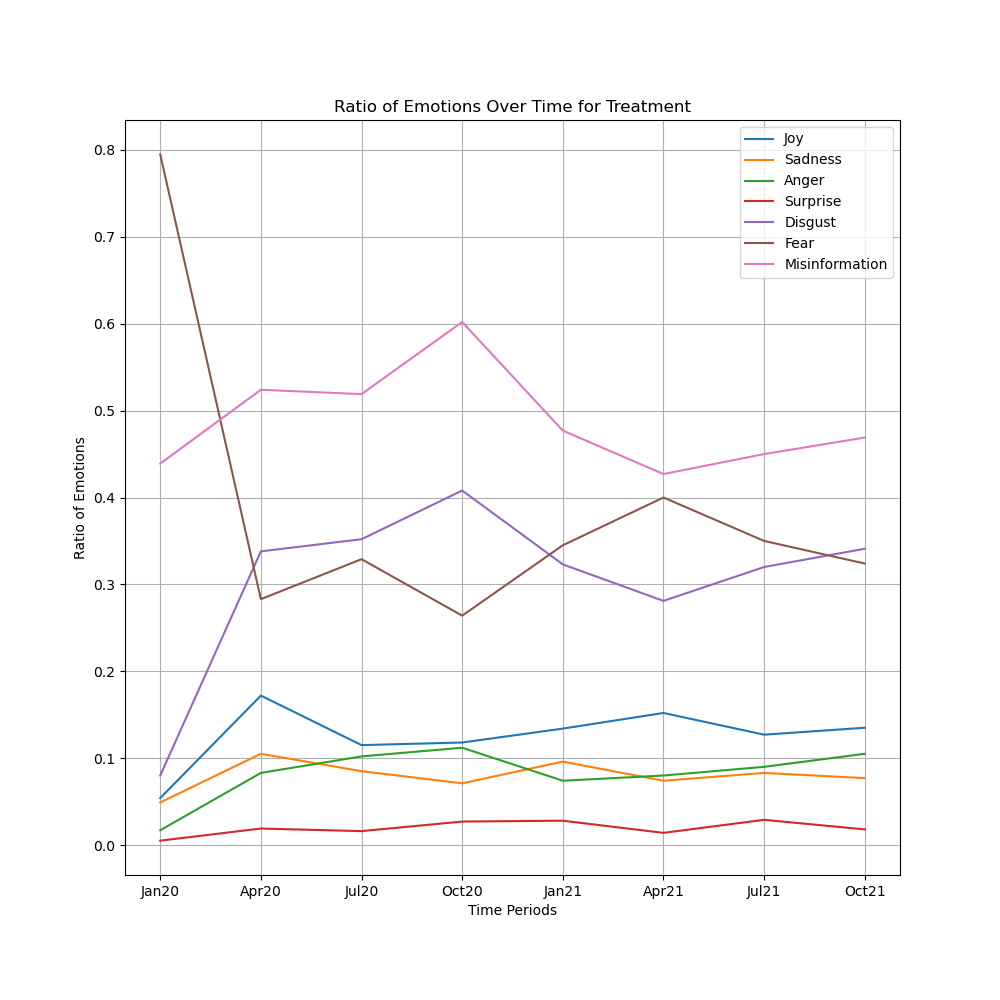
\includegraphics[width=\textwidth]{images/TreatmentEmotion.png}
\captionof{figure}{Ratios of Emotions and Misinformation for Treatment}
\label{fig:treatemo}
\end{minipage}
\end{figure}

\begin{figure}[H]
\begin{minipage}[c]{0.49\linewidth}
\centering
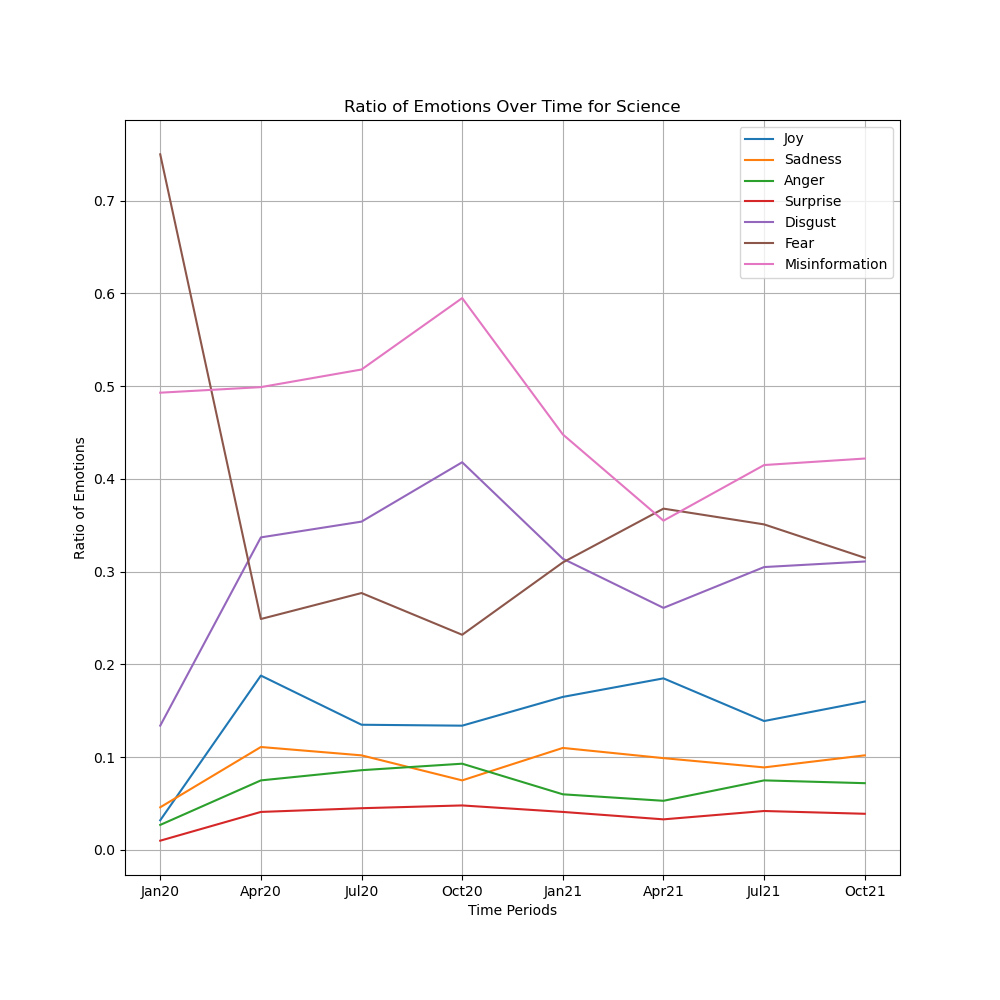
\includegraphics[width=\textwidth]{images/ScienceEmotion.png}
\captionof{figure}{Ratios of Emotions and Misinformation for Science}
\label{fig:sciemo}
\end{minipage}
\begin{minipage}[c]{0.49\linewidth}
\centering
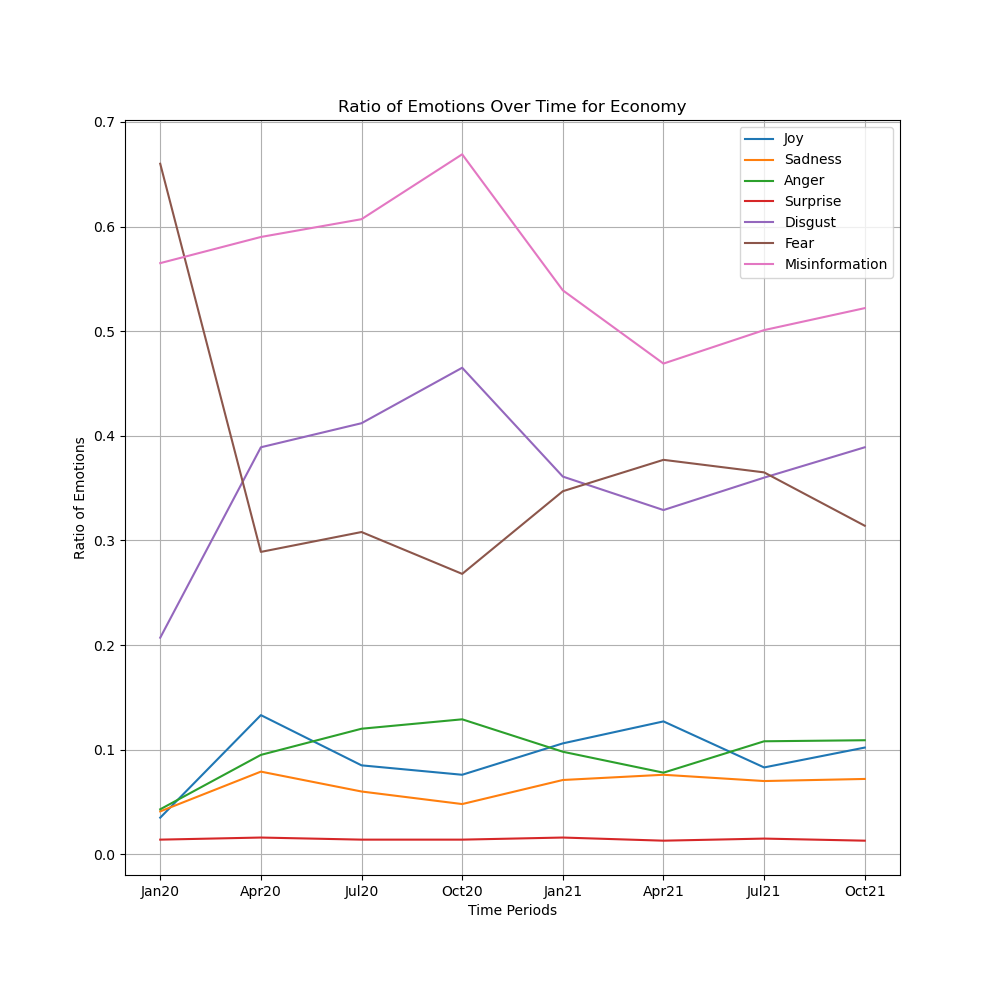
\includegraphics[width=\textwidth]{images/EconomyEmotion.png}
\captionof{figure}{Ratios of Emotions and Misinformation for Economy}
\label{fig:ecoemo}
\end{minipage}
\end{figure}

\begin{figure}[H]
\begin{minipage}[c]{0.49\linewidth}
\centering
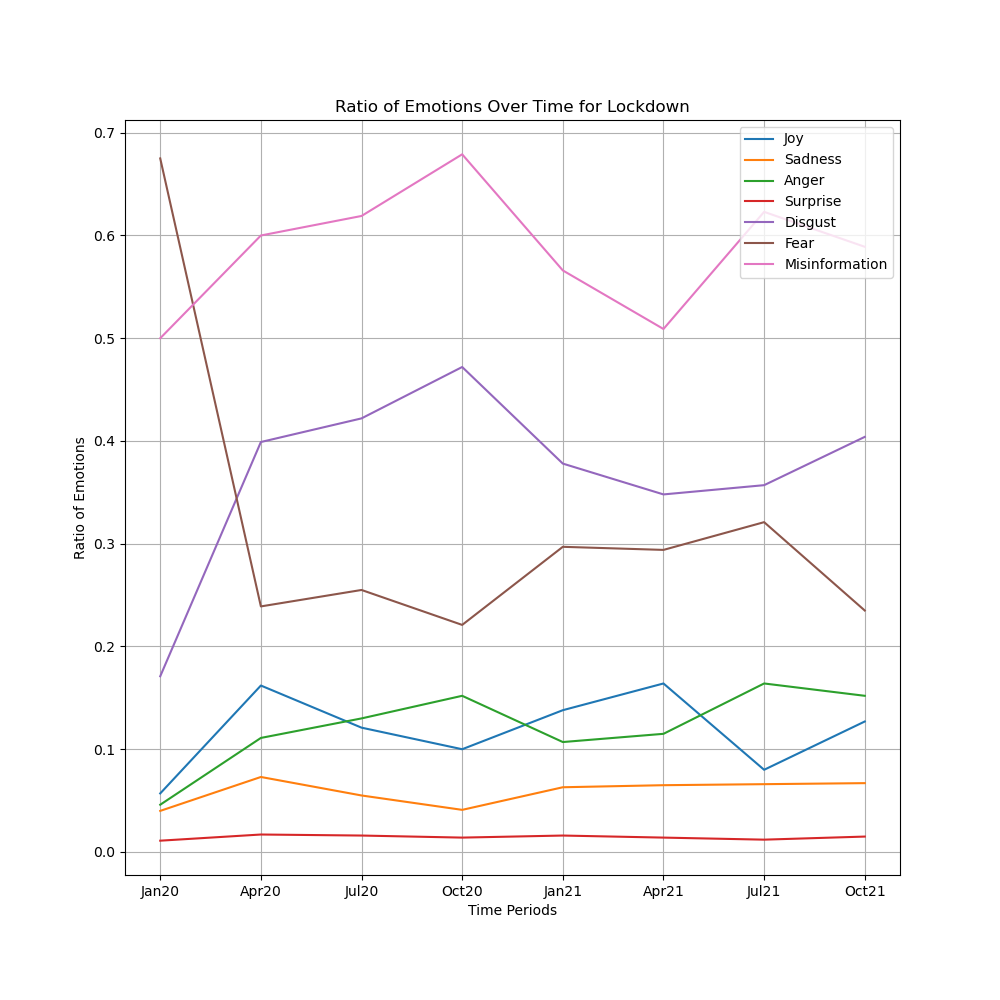
\includegraphics[width=\textwidth]{images/LockdownEmotion.png}
\captionof{figure}{Ratios of Emotions and Misinformation for Lockdown}
\label{fig:lockemo}
\end{minipage}
\begin{minipage}[c]{0.49\linewidth}
\centering
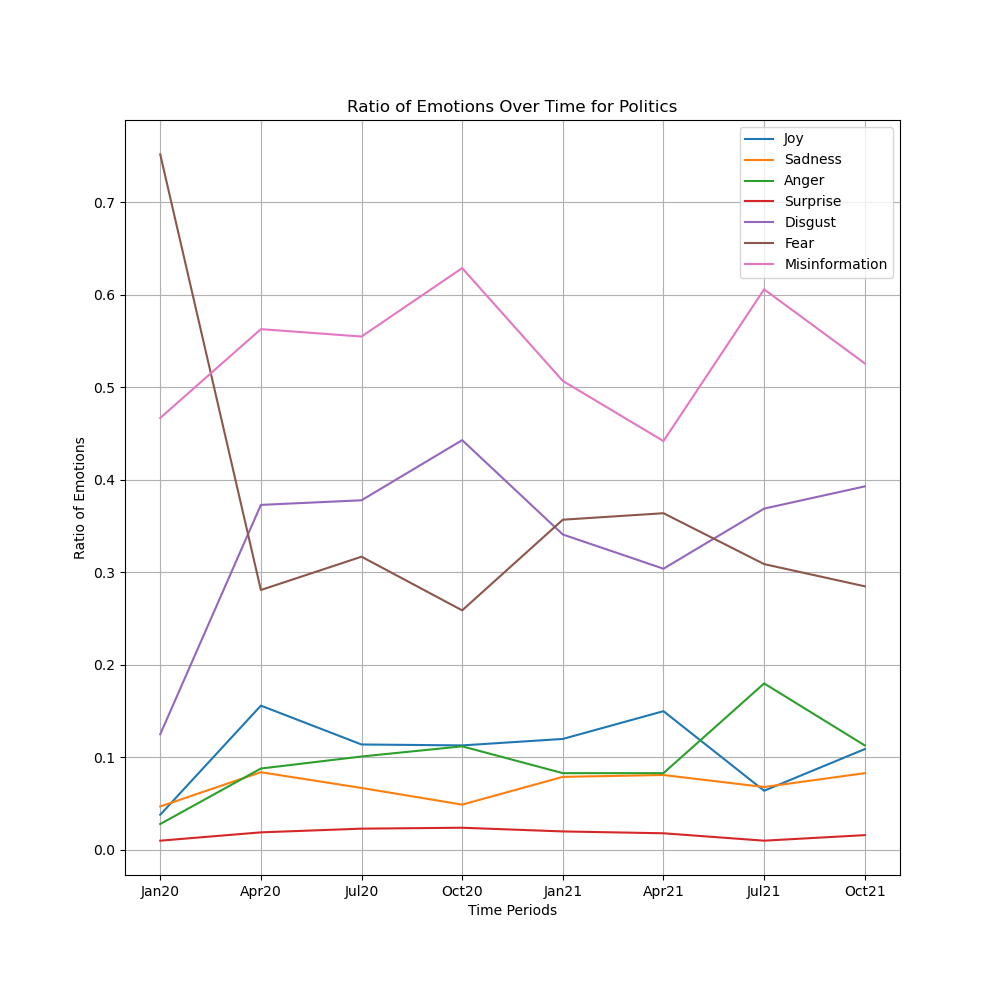
\includegraphics[width=\textwidth]{images/PoliticsEmotion.png}
\captionof{figure}{Ratios of Emotions and Misinformation for Politics}
\label{fig:polemo}
\end{minipage}
\end{figure}

\end{appendices}

%==================================================================================================================================
%   BIBLIOGRAPHY   

% The bibliography style is agsm (Harvard)
% The bibliography always appears last, after the appendices.

\bibliographystyle{agsm}

% Force the bibliography not to be numbered
\renewcommand{\thechapter}{0} 
\bibliography{l4proj}

\end{document}
